\documentclass[11pt,letterpaper]{article}
\pdfoutput=1
\usepackage{jheppub}
\usepackage{mathtools,amssymb,amsthm,bm,booktabs,adjustbox}
\setlength{\emergencystretch}{2em}
\newcommand{\RR}{\mathbb R}
\newcommand{\CC}{\mathbb C}
\newcommand{\ZZ}{\mathbb Z}
\newcommand{\OO}{\mathcal O}
\newcommand{\dbar}{\bar\partial}
\newcommand{\Cone}{\mathcal C}
\newcommand{\HH}{\mathsf H}
\newcommand{\BF}{B_F}
\newcommand{\BR}{B_R}
\newcommand{\gKS}{g^{\mathrm{KS}}}
\newcommand{\gC}{g_{\Cone}}
\newcommand{\Oformal}{O_{\mathrm{formal}}}
\DeclareMathOperator{\tr}{tr}
\DeclareMathOperator{\Tr}{Tr}
\DeclareMathOperator{\End}{End}
\DeclareMathOperator{\Hom}{Hom}
\DeclareMathOperator{\Ext}{Ext}
\DeclareMathOperator{\Vol}{Vol}
\DeclareMathOperator{\Rm}{Rm}
\DeclareMathOperator{\SU}{SU}
\DeclareMathOperator{\U}{U}
\DeclareMathOperator{\SO}{SO}
\DeclareMathOperator{\PU}{PU}

\newtheorem{theorem}{Theorem}[section]
\newtheorem{proposition}[theorem]{Proposition}
\newtheorem{lemma}[theorem]{Lemma}
\theoremstyle{remark}
\newtheorem{remark}[theorem]{Remark}
\title{Light vectors and scalar interactions near heterotic K3 gauge enhancement}
\author{Bernd Johannes Wuebben}
\affiliation{New York, NY, USA}
\emailAdd{wuebben@gmail.com}
\date{November 8, 2026}
\subheader{November 8, 2026\\This version: November 8, 2026}
\abstract{We prove a uniform comparison for a four-scalar tree amplitude
near gauge enhancement in a smooth $SO(32)$ heterotic K3 compactification.
A rank-six stable-bundle family approaches the direct sum of two
isomorphic stable rank-three bundles. Two
harmonic deformation amplitudes $a,b$ give three squared Higgs masses
proportional to $b^2$, $a^2$ and $a^2+b^2$.
For two specified massless bundle scalars, the complete leading
Yang--Mills amplitude, including all internal vector and scalar
Kaluza--Klein modes, approaches an explicit light-vector exchange formula.
The absolute error is quadratic in the deformation amplitudes, uniformly as $b/a$
tends to zero, below the heavier Higgs masses and away from the light
poles. Harmonic orthogonality controls the actual cubic vertices, while
an exact scalar contact--exchange cancellation removes inverse-mass losses.
The same estimates give inverse-square growth of the sectional curvature
of the harmonic bundle-moduli metric on a selected plane, with uniform
relative error. We also obtain a
ratio-uniform relative bound for the first-order coupled vector equation
and a fixed-ray coefficient with a Pauli selection rule. At the next
tree order we control quadratic potential mixing with K3 metric deformations and
compute the universal graviton exchange. The complete coefficient at that
order and a finite-string-scale remainder remain open.}
\keywords{Superstrings and Heterotic Strings, Compactification and String Models,
Supersymmetric Effective Theories}
\hypersetup{pdftitle={Light vectors and scalar interactions near heterotic K3 gauge enhancement},
pdfauthor={Bernd Johannes Wuebben}}
\begin{document}
\maketitle
\section{Introduction}\label{sec:introduction}

Gauge enhancement in a heterotic compactification occurs when the internal
connection acquires additional parallel adjoint sections. A deformation away
from that locus makes the corresponding external vectors massive. The
finite-dimensional Higgs mass matrix describes the leading mechanism, but
an absolute error estimate need not resolve its smallest eigenvalue: several
Higgs scales can approach zero at unrelated rates. There is a related
problem for scalar interactions. A comparison of kinetic metrics does not,
by itself, control the derivatives entering their curvature or identify the
curvature of a bundle-moduli subspace with a coupling in the full reduced
theory.

We address these questions on one family of smooth K3 compactifications of
the $\operatorname{Spin}(32)/\ZZ_2$ heterotic theory with vector structure.
We use $\SO(32)$ for its gauge algebra and its real vector-bundle
description. The background bundle contains two identical stable
rank-three factors at the enhancement point. Two orthonormal harmonic
deformation coordinates, with coefficients $a,b$, break the multiplicity
$\SU(2)$. The K3 surface remains smooth and its polarization is fixed.
The moment maps vanish throughout this bundle enhancement; no nonzero
Fayet--Iliopoulos parameter is varied.

Let $g_0$ be the fixed reference K3 metric, $V_0=\Vol(g_0)$, and let
$L^2g_0$ be the physical internal metric at leading order. The three leading
squared vector masses obey
\begin{equation}\label{eq:intro-masses}
 m_j^{2,(0)}=\widehat m_j^2\bigl(1+O(a^2+b^2)\bigr),\qquad
 (\widehat m_1^2,\widehat m_2^2,\widehat m_3^2)
 =\frac{8}{3V_0L^2}(b^2,a^2,a^2+b^2),\quad 0<b\le a.
\end{equation}
The error is proportional to each individual squared mass, with a
constant independent of $b/a$. In particular, at
$a=\varepsilon$, $b=\varepsilon^p$, $p>1$, the weakest squared mass
has order $\varepsilon^{2p}/L^2$, while its relative geometric error
still has order $\varepsilon^2$. This is a statement about actual
Hermitian--Einstein connections, obtained by applying the quantitative
local comparison of \cite{wuebben15} to the compactification family.
The Pauli-matrix eigenvalues alone would not give this conclusion.

We also calculate the first coefficient of the coupled tree-level vector
equations. Write $\eta=\alpha'/L^2$. Eliminating the complete leading
metric and two-form vector towers gives a finite, energy-dependent pencil
$F^{[1]}(\lambda,\eta)$, defined in section~\ref{sec:coupled}.
Its three positive roots, converted to squared masses by $L^{-2}$,
satisfy
\begin{equation}\label{eq:intro-corrected}
 \left|\frac{m_j^{2,[1]}}{\widehat m_j^2}-1\right|
 \le C\left(a^2+b^2+\frac{\eta}{b^2}\right).
\end{equation}
An anti-self-dual (ASD) Hodge identity checks the relative coefficients of the two
mixings and proves positivity and preservation of the unbroken kernels.
The sufficient region $\eta=o((a^2+b^2)b^2)$ makes this calculated
correction smaller than the geometric relative error. Equation
\eqref{eq:intro-corrected} concerns the defined pencil; it does not
bound an uncomputed remainder in exact string poles.

The second physical quantity is a neutral-scalar interaction. In the same
holomorphic local quotient chart, the actual harmonic metric has a
relative quadratic comparison with the hyperk\"ahler cone metric.
Ricci-flat K\"ahler regularity upgrades this comparison to every fixed
derivative order on compact smooth angular regions. An explicit
horizontal two-plane has cone sectional curvature $3/(2b^2)$.
We solve the mixed Einstein and two-form constraints, account for the
other neutral fields and for the small axion kinetic block, and obtain
the leading physical sectional curvature
\begin{equation}\label{eq:intro-curvature}
 \mathcal K_{\rm phys}^{\rm lead}
 =\frac{3g_{10}^2}{4L^2\kappa^2\varepsilon^2}
       \bigl(1+O_\kappa(\varepsilon^2)\bigr),\qquad
 a=\varepsilon,\quad b=\kappa\varepsilon,\quad 0<\kappa\le1.
\end{equation}
Here $g_{10}$ is defined by the gauge action in
section~\ref{sec:vectors}. This coefficient multiplies a specified
two-polarization quartic interaction in scalar normal coordinates.
Its derivation first extracts the tree-level large-volume coefficient
on a fixed regular patch, then takes the displayed geometric limit.
It is not uniform as $\kappa\to0$. Eliminating the Higgs multiplets
requires probe energies much smaller than $b/L$.

Heterotic bundle stability, charged fields and D-term Higgsing have an
established effective-theory description \cite{stabilitywalls}.
The $\SO(32)$ embedding, spectrum and abelian mass criteria used here
follow the K3 analysis of \cite{honecker}. Bundle and matter metrics
were computed in \cite{louis}, while the general geometry--bundle--two-form
fibration and its large-volume hierarchy were developed in
\cite{alpv}. We retain the compensator and curvature-squared terms needed
to identify the leading coefficient; we do not import a specialized
duality completion as the metric of the present compactification.
The relation between scalar curvature and covariant amplitudes is also
standard \cite{cheung}.

Universal heterotic representatives and higher-order moduli metrics are
developed in \cite{candelas,mcorist_sticka_svanes,mcorist_yin}.
Their Calabi--Yau threefold results concern four-dimensional
compactifications; we use the action and covariant-variation conventions,
not their moduli-metric theorems as results for six-dimensional K3 vacua.

The quantitative input is the energy-relative spectral and quotient-metric
comparison in \cite{wuebben15}. We use the local harmonic quadraticity
argument of \cite{wuebben20} without extending that paper's global
compactness theorem to this family. The new application combines those
inputs with a compact heterotic model, the coupled vector calculation,
and a physically normalized curvature coefficient on that same family.
The Hodge identity, interior estimates and quotient curvature formula
are standard mechanisms or direct calculations. Their role is to make
the physical identifications and their accuracy precise.

Section~\ref{sec:compactification} constructs the family and fixes its
local coordinates. Sections~\ref{sec:vectors} and~\ref{sec:coupled}
derive the vector statements and the retained field content.
Sections~\ref{sec:derivatives} and~\ref{sec:scalar} establish the
derivative estimates and the leading ambient scalar interaction.
Throughout, the string coupling is taken in the tree regime independently
of the geometric parameters.

\section{The compactification and its enhancement locus}\label{sec:compactification}

\subsection{Stable factors and the orthogonal embedding}
Fix a smooth projective K3 surface $S$ with $\operatorname{Pic}(S)=\ZZ H$,
where $H$ is ample. Let $g_0$ be its Ricci-flat K\"ahler metric in that
class, oriented so that primitive $(1,1)$ forms are anti-self-dual. Norms
and harmonic representatives without an explicit scale use $g_0$ and
unnormalized trace inner products. Write $V_0=\Vol(S,g_0)$.

Choose locally free $\mu_H$-stable bundles $A,B$ with
\begin{equation}\label{eq:factors}
 \begin{gathered}
 \operatorname{rk}A=\operatorname{rk}B=3,\qquad \det A=\det B=\OO_S,\\
 c_2(A)=7,\quad c_2(B)=10,\qquad A\not\simeq A^*,\quad B\not\simeq B^*.
 \end{gathered}
\end{equation}
Here existence includes the locally free, slope-stable and non-self-dual
conditions. We give the argument because these conditions determine both
the analytic application and the unbroken gauge algebra.

For $k=7,10$ the Mukai vector is $v_k=(3,0,3-k)$, with
$v_7^2=24$ and $v_{10}^2=42$. Both vectors are primitive. An equal
reduced-Hilbert-polynomial proper subsheaf would have first Chern class
zero and Euler characteristic divided by rank equal to $-1/3$ or
$-4/3$. Neither is possible for rank one or two. Thus $H$ is general
for these vectors. Yoshioka's nonemptiness and irreducibility theorem,
together with the slope-stability and local-freeness criteria in
\cite[Theorem~0.1, Proposition~0.5 and section~3.3]{yoshioka}, gives
nonempty slope-stable and locally free opens. In that notation the
integer $l$ equals three and $v_k^2\ge2l^2$. The exceptions to the
locally free criterion do not occur: the vectors have rank three,
whereas the spherical exception of the form
$(\operatorname{rk}v_0)v_0-\omega$ would have square rank.
Irreducibility makes the two opens intersect. Since $\operatorname{Pic}^0(S)=0$,
their determinant is trivial.

Dualization acts holomorphically as an involution on this smooth open.
At a fixed point $F$, simplicity makes an isomorphism $F\to F^*$
symmetric or skew-symmetric after scalar normalization. Odd rank
excludes the latter. The invariant tangent space is
$H^1(S,\mathfrak{so}(F))\simeq H^1(S,F)$: use
$\Lambda^2F^*\simeq F$ and the symmetric form. Stability and Serre
duality give $H^0(F)=H^2(F)=0$, and Riemann--Roch gives
\begin{equation}\label{eq:selfdual-dim}
 h^1(F)=k-6,\qquad h^1(\End F)=6k-16.
\end{equation}
The fixed locus of a holomorphic involution is smooth with its invariant
tangent space. One can see this directly by replacing local coordinates
$z$ centered at a fixed point by
$\tfrac12(z+D\iota_0\,z\circ\iota)$; their derivative is the
identity and the action becomes linear. The fixed locus therefore
cannot fill the stable locally free open. This proves that the choices
in \eqref{eq:factors} exist. Their distinct second Chern classes also
exclude isomorphisms between $A$ or $A^*$ and $B$ or $B^*$.

At enhancement set $E_0=A\otimes\CC^2$ and define the real gauge
bundle
\begin{equation}\label{eq:gauge-bundle}
 \mathcal V=(E_0\oplus B)_{\RR}\oplus\RR^{14},\qquad
 \mathcal V\otimes\CC=E_0\oplus E_0^*\oplus B\oplus B^*\oplus\OO^{14}.
\end{equation}
It has real rank 32, $w_2(\mathcal V)=0$, and
$p_1(\mathcal V)=-2c_2(E_0\oplus B)=-48=p_1(TS)$.
The weighted instanton number is
\begin{equation}\label{eq:instanton}
 2c_2(A)+c_2(B)=2\cdot7+10=24.
\end{equation}
There is consequently no five-brane source in the integrated Bianchi
identity \cite{honecker}. The Donaldson--Uhlenbeck--Yau correspondence
\cite{donaldson,uy} supplies determinant-flat HE connections, which are
ASD on $S$. They give the leading background with eight supercharges,
or six-dimensional $\mathcal N=(1,0)$ supersymmetry. Equation
\eqref{eq:instanton} is an integrated condition; it does not set the
gauge and tangent curvature densities equal pointwise. Their difference
sources the first correction in section~\ref{sec:coupled}.

The parallel orthogonal adjoint sections have compact algebra
\begin{equation}\label{eq:centralizer}
 \mathfrak h_0=\mathfrak{so}(14)\oplus\mathfrak u(2)\oplus\mathfrak u(1),
 \qquad \dim_\RR\mathfrak h_0=96.
\end{equation}
Indeed the endomorphism blocks give $\End(\CC^2)$ and $\CC$ by
simplicity. The additional exterior-square blocks have no parallel
sections. For example,
\[
 \Lambda^2(A\otimes\CC^2)=
 (\Lambda^2 A\otimes\operatorname{Sym}^2\CC^2)
 \oplus(\operatorname{Sym}^2 A\otimes\Lambda^2\CC^2),
\]
and $H^0(A\otimes A)=\Hom(A^*,A)=0$ by stability and
non-self-duality. The other cross blocks vanish for the same reason.
There are no maps to the trivial fourteen-dimensional factor.
This also explains why replacing $A$ by a pseudoreal rank-two factor
would give a different centralizer. All central factors here have
$c_1=0$; the abelian flux mass matrix of \cite[section~3.2]{honecker}
vanishes. Protection of the nonconstant-profile vector calculation
requires the separate argument in section~\ref{sec:coupled}.

\subsection{Harmonic coordinates and actual bundles}\label{subsec:harmonic}
General K3 formality results \cite{budurzhang} identify quadratic
deformation germs. The quantitative metric application below needs
the stronger coordinate specification in the original harmonic chart.

The harmonic space $H^1(S,\End A)$ has complex dimension 26 and a
quaternionic structure. Choose thirteen orthonormal symplectic pairs,
normalized using the parallel holomorphic two-form. Then
\[
 H^1(S,\End E_0)=H^1(S,\End A)\otimes\End(\CC^2)
\]
has coordinates $(X_j,Y_j)_{j=1}^{13}$ with the flat real metric
\begin{equation}\label{eq:flatmetric}
 \|\dot x\|^2=\operatorname{Re}\sum_{j=1}^{13}
 \tr(\dot X_j^*\dot X_j+\dot Y_j^*\dot Y_j).
\end{equation}
The multiplicity group acts by simultaneous conjugation; its center
acts trivially. The complex and real moment equations are
\begin{equation}\label{eq:moments}
 \sum_j[X_j,Y_j]=0,\qquad
 \sum_j\bigl([X_j,X_j^*]+[Y_j,Y_j^*]\bigr)=0.
\end{equation}
Only their zero level is used. Let $\Cone$ be this hyperk\"ahler
quotient by the effective group $\PU(2)$, with metric $\gC$ on its
smooth-simple part.

We record why these are exact local deformation coordinates, rather
than merely the quadratic part of an unspecified obstruction. Put
$d=\dbar_{E_0}$ and denote harmonic projection and Green operators
by $H_q,G_q$. The convergent harmonic recursion of
\cite[Lemma~2.1]{wuebben15} is
\begin{equation}\label{eq:recursion}
 \mathfrak a(x)=x-d^*G_2(\mathfrak a(x)\wedge\mathfrak a(x)),\qquad
 \mathfrak k(x)=H_2(\mathfrak a(x)\wedge\mathfrak a(x)).
\end{equation}
On a Ricci-flat K3 its obstruction is exactly
\begin{equation}\label{eq:quadratic}
 \mathfrak k(x)=H_2(x\wedge x).
\end{equation}
For completeness, a harmonic $\End E_0$-valued $(0,2)$-form is
$\xi\bar\sigma$ with $\xi$ parallel. This follows from the formula
for $d^*(\xi\bar\sigma)$ and the Bochner identity on the
zero-mean-curvature endomorphism bundle. If $d^*u=0$ and
$\gamma=\phi\bar\sigma$, the coefficients of
$u\wedge d^*\gamma$ and $d^*\gamma\wedge u$ are, up to common
nonzero scalars,
$-\sum_j u_{\bar j}\nabla_j\phi$ and
$\sum_j(\nabla_j\phi)u_{\bar j}$. Pair either with a parallel
$\xi$ and integrate by parts, keeping the matrix order. The resulting
terms contain $\sum_j\nabla_j u_{\bar j}=-d^*u$ and vanish.
Consequently both products have zero harmonic projection.
Writing $\mathfrak a=x+\beta$ with $\beta$ coexact and
$d^*$-closed eliminates all terms containing $\beta$ in the
obstruction and proves \eqref{eq:quadratic}. This is precisely the
local argument in \cite[Lemma~3.1]{wuebben20}; it uses none of that
paper's later global rank or no-bubbling hypotheses.

Serre duality identifies \eqref{eq:quadratic} with the first equation
in \eqref{eq:moments}; a common nonzero symplectic factor and the
rank-dual identification do not change its zero set. Fixing the
determinant removes no harmonic directions because $H^1(S,\OO)=0$.
The analytic quotient construction \cite{buchdahl} and HE reconstruction
\cite[Theorem~1.1]{wuebben15} therefore identify the balanced quotient
with the actual nearby HE moduli. This identification $\Psi$ is
holomorphic in these same coordinates: the holomorphic classifying
map and the reconstructed HE map assign the same bundle class to
each harmonic deformation. No further nonlinear reparametrization
is made.

The quantitative input, specialized to this fixed background, is
\begin{equation}\label{eq:metriccomparison}
 (1-Cr^2)\gC\ \le\ \Psi^*\gKS\ \le\ (1+Cr^2)\gC,
 \qquad r=\|x\|,
\end{equation}
on genuine smooth stratum tangents. Here $\gKS$ is the real harmonic
Kodaira--Spencer metric in the unnormalized Dolbeault norm. The same
constant works when positive orbit scales have arbitrary ratios. It
may depend on the fixed metric, bundles, ranks, harmonic dimensions
and elliptic gaps. This does not assert uniformly sized smooth
coordinate charts through every lower stratum. On the smooth-simple
locus $\gKS$ is hyperk\"ahler \cite{itoh}.

Let $\sigma_j$ be the Pauli matrices with
$\tr(\sigma_i\sigma_j)=2\delta_{ij}$ and
$[\sigma_i,\sigma_j]=2i\epsilon_{ijk}\sigma_k$. Our family is
\begin{equation}\label{eq:pauli}
 X_1=a\sigma_3,\qquad X_2=b\sigma_1,\qquad
 X_j=0\ (j\ge3),\qquad Y_j=0,\qquad a,b\in\RR.
\end{equation}
It satisfies both moment equations since its nonzero matrices are
Hermitian. If $ab\ne0$, a line invariant under $\sigma_3$ is an
eigenline, and $\sigma_1$ exchanges the two eigenlines. The
representation is therefore simple. Reconstruction gives an actual
stable rank-six bundle $E_{a,b}$ with $c_2=14$ and trivial determinant.
The local simple moduli space has complex dimension
$104-2\cdot3=98$.

On a nonzero axis the representation is the sum of two distinct
characters, corresponding to two nearby stable rank-three factors.
Upper semicontinuity preserves the other Hom vanishings after
shrinking the neighborhood. The unbroken algebra is thus
$\mathfrak{so}(14)\oplus\mathfrak u(1)^2$ generically,
$\mathfrak{so}(14)\oplus\mathfrak u(1)^3$ on an axis, and
\eqref{eq:centralizer} at the origin. Their dimensions are
93, 94 and 96, respectively.

\section{Light vectors and the retained spectrum}\label{sec:vectors}

\subsection{The physical vector operator}
On real skew-adjoint generators set
$\BF(U,V)=-\tfrac12\Tr_{32}(UV)$. Define $g_{10}$ by
\begin{equation}\label{eq:YMaction}
 S_{\rm YM}=-\frac1{4g_{10}^2}\int
    \BF(F_{MN},F^{MN})\,d\Vol_{10}.
\end{equation}
The constant dilaton is absorbed in this coupling. Initially use the
product spacetime metric $g_{1,5}+L^2g_0$; a constant change to
six-dimensional Einstein frame must rescale masses and scalar kinetic
tensors consistently. On a realified unitary block $\BF$ restricts to
$-\operatorname{Re}\Tr$. A multiplicity generator at $E_0$ consequently
has reference norm $3V_0\tr_2(\xi^*\xi)$.

For a Lorentz-transverse external fluctuation
$\delta\mathcal A_\mu=v_\mu\psi(y)$, background gauge separates the
internal Goldstone variation. The external kinetic and mass forms are
$g_{10}^{-2}\|\psi\|^2_{L^2(L^2g_0)}$ and
$g_{10}^{-2}\|d_{\mathcal A}\psi\|^2_{L^2(L^2g_0)}$.
The coupling cancels in their generalized eigenvalue. On endomorphism
zero-forms the HE K\"ahler identity gives
\begin{equation}\label{eq:physicaloperator}
 d_{\mathcal A}^*d_{\mathcal A}=2\Delta_{\dbar,\End E}.
\end{equation}
The induced endomorphism mean curvature is zero, so the $\partial$
and $\dbar$ Laplacians agree in this degree. This is a
zero-form vector-profile identity, not an identity for the full
one-form Yang--Mills Hessian; compare \cite[appendix~A]{louis}.
The zero-form and one-form norms scale as $L^4$ and $L^2$,
respectively, so physical squared masses acquire the factor $L^{-2}$.

For $\xi=\sum z_j\sigma_j$ the finite Dolbeault energy and mass are
\begin{align}
 q_x(\xi)&=\sum_j\|[\xi,X_j]\|^2+\|[\xi,Y_j]\|^2
 =8\bigl(a^2|z_1|^2+(a^2+b^2)|z_2|^2+b^2|z_3|^2\bigr),
 \label{eq:pauli-energy}\\
 M_0(\xi)&=3V_0\tr(\xi^*\xi)=6V_0\sum_j|z_j|^2.
 \label{eq:pauli-mass}
\end{align}
Thus its ordered eigenvalues for $0<b\le a$ are
$\tfrac4{3V_0}(b^2,a^2,a^2+b^2)$.

\begin{proposition}\label{prop:vectors}
For the actual bundles of \eqref{eq:pauli}, sufficiently near the
origin, there are exactly three real vector species whose positive
masses tend to zero away from the unbroken kernel. They satisfy
\eqref{eq:intro-masses}, with a constant independent of $b/a$.
The corresponding two-sided inequality retains exact zeros on the
axes and at the origin. All other nonzero vector-profile eigenvalues
have a fixed positive lower bound in reference units.
\end{proposition}
\begin{proof}
Apply \cite[Theorem~1.1(ii)]{wuebben15} at the locally free polystable
bundle $A\otimes\CC^2$, at constant polarization and fixed
determinant. Its trace-free multiplicity algebra has dimension three.
The theorem bounds every small Dolbeault eigenvalue between
$(1-C\|x\|^2)\nu_j(x)$ and $(1+C\|x\|^2)\nu_j(x)$,
including zeros, and gives a positive complementary gap. Here
$\|x\|^2=2(a^2+b^2)$ and \eqref{eq:pauli-energy}--\eqref{eq:pauli-mass}
give $\nu_j$. Equation~\eqref{eq:physicaloperator} and the internal
scale give \eqref{eq:intro-masses}. The real adjoint sector is preserved
by this Laplacian. Each complex eigenspace is the complexification of
its Hermitian, or equivalently skew-Hermitian, real form. Its complex
multiplicity is therefore the number of real generator profiles,
not twice that number. The remaining orthogonal-adjoint blocks have
the kernels already identified in \eqref{eq:centralizer}; their
positive spectrum stays separated from zero by elliptic continuity
on the fixed compact background.
\end{proof}

The essential input is the relative form of the imported estimate.
In its proof the complementary Schur term is bounded by the finite
energy of the same vector. A uniform additive error of order
$(a^2+b^2)^2$ would not establish the result when $b\ll a^2$.
There is no additional gauge coupling multiplying the masses in
\eqref{eq:intro-masses} after the convention \eqref{eq:YMaction} is fixed.

\subsection{Massless fields and Higgs multiplets}
The vector gap does not make the remaining matter heavy. The full
orthogonal adjoint decomposes into endomorphism, exterior-square,
mixed tensor and fourteen-dimensional vector sectors. For a stable
determinant-trivial rank-$r$ bundle $F$ with $c_2(F)=k$ and the
Hom vanishings established above, Riemann--Roch and Serre duality give
\begin{align}\label{eq:cohomology}
 h^1(F)&=k-2r,&
 \dim_{\mathbb H}\mathcal M_F&=rk-r^2+1,\\
 h^1(F\otimes G)&=r_Gk_F+r_Fk_G-2r_Fr_G,&
 h^1(\Lambda^2F)&=(r-2)k-r(r-1).\nonumber
\end{align}
These follow by integrating $\operatorname{ch}(\cdot)\operatorname{td}(S)$;
the exterior-square formula uses
$c_2(\Lambda^2F)=(r-2)c_2(F)$ when $c_1(F)=0$.
The neutral moduli formula follows from $h^1(\End F)=2rk-2r^2+2$.
In the spectrum convention of \cite{honecker}, complex conjugate
sectors combine into full hypermultiplets. At a generic point the
dimension-weighted counts are listed in table~\ref{tab:matter}.

\begin{table}[t]
\centering
\caption{Generic massless hypermultiplet contributions. Charges refer to
the two central $\U(1)$ factors. The fourteen-dimensional sectors contain
hypermultiplets in the vector representation of $\SO(14)$, not additional
gauge vectors.}\label{tab:matter}
\begin{adjustbox}{max width=\textwidth,center}
\begin{tabular}{lr}
\toprule
Sector & Dimension-weighted hypermultiplet count\\
\midrule
$E$ moduli, neutral &49\\
$B$ moduli, neutral &22\\
$\Lambda^2E$, charge $(2,0)$ &26\\
$\Lambda^2B$, charge $(0,2)$ &4\\
$E\otimes B$, charge $(1,1)$ &66\\
$E\otimes B^*$, charge $(1,-1)$ &66\\
$E$ sector in $\mathbf {14}$, charge $(1,0)$ &28\\
$B$ sector in $\mathbf {14}$, charge $(0,1)$ &56\\
K3 geometry and two-form fields &20\\
\midrule
Total &337\\
\bottomrule
\end{tabular}
\end{adjustbox}
\end{table}

At enhancement the $E$ endomorphism sector consists of thirteen
adjoint-$\U(2)$ hypermultiplets and contributes 52. On a nonzero axis
the two distinct rank-three factors contribute $2\cdot13$ neutral
hypermultiplets and 24 off-diagonal charged ones, giving 50.
The other dimension-weighted totals are unchanged. Thus
\begin{equation}\label{eq:counts}
 (n_H,n_V)=
 \begin{cases}
 (340,96),&a=b=0,\\
 (338,94),&ab=0,\quad a^2+b^2>0,\\
 (337,93),&ab\ne0.
 \end{cases}
\end{equation}
There is one tensor multiplet, containing the six-dimensional dilaton,
and the gravity multiplet. Every row obeys
$n_H-n_V+29n_T=273$. This is a gravitational anomaly count; it does
not replace the gauge-anomaly and embedding analysis of \cite{honecker}.
As a separate index check, the real gauge ASD complex has
$h^1-h^0-h^2=4\cdot30\cdot24-4\cdot496=896$ on K3. Our generic
gauge hypermultiplets contribute $4(337-20)$, and $h^0=93$ gives
$4(337-20)-4\cdot93=896$; the corresponding enhanced and axis
counts agree as well. Here the expression subtracts all four
parallel contributions, equivalently using $h^2=3h^0$ in the
ASD index.

Three hypermultiplets and three vectors combine into three massive
$\mathcal N=(1,0)$ vector multiplets generically. Each massive vector
has five physical polarizations and three physical real scalar
partners; the fourth scalar of its hypermultiplet is a Goldstone
mode. On an axis only two such multiplets are massive.

\subsection{The common low-energy space}
Choose background gauge, diffeomorphism gauge and two-form gauge at
the reference background. The leading internal operators are the
adjoint zero-form Laplacian for vectors, the positive ASD deformation
square for connection scalars, the physical Lichnerowicz operator for
metric deformations, ordinary Hodge Laplacians for forms, and the
corresponding Dirac complexes for fermions. The ASD square is
$d_{\mathcal A}d_{\mathcal A}^*+2d_{\mathcal A}^{+*}d_{\mathcal A}^+$
on one-forms. The parallel-spinor factorization gives nonnegativity
of the physical Ricci-flat metric operator \cite{parallelspinor};
this excludes the unphysical Euclidean conformal mode. Compactness
gives finite kernels and positive complementary gaps. Supersymmetry
identifies the physical superpartners.

Take a cutoff below the minimum of these reference gaps and retain
every reference low mode, including the gauge/Goldstone complex.
Smooth elliptic dependence gives common finite low spectral clusters
and a complementary gap $\gamma>0$ for all sufficiently small
$(a,b)$. One must not first divide out a different number of scalar
gauge directions at each stratum and then assert continuity on a
fixed space. The theory with the Higgs multiplets retained has the
common leading window $E_{\rm probe}\ll\sqrt\gamma/L$.
Eliminating them instead requires $E_{\rm probe}\ll b/L$ on a
generic regular patch. Higher-derivative string terms are used
perturbatively through leading resolvents, not as a positive
second-order operator on the entire tower.

\section{The first coupled vector correction}\label{sec:coupled}

\subsection{Action convention and the corrected background}
For this calculation use unit-scale internal coordinates and remove the
common gravitational prefactor. Set $\eta=\alpha'/L^2$ and use positive
forms $\BF=-\tfrac12\Tr_{32}$ and $\BR=-\tfrac12\Tr_T$ on
the compact gauge and internal Euclidean rotation algebras. The
Lorentzian extension of the tangent trace is understood in the
ten-dimensional action. Our convention is
\begin{equation}\label{eq:heterotic-action}
 \begin{split}
 S=\int e^{-2\Phi}\sqrt{-G}\Bigl[&
 R+4|d\Phi|^2-\frac1{12}H_{MNP}H^{MNP}\\
 &-\frac\eta4\bigl(\BF(F_{MN},F^{MN})-\BR(R_{MN},R^{MN})\bigr)
 \Bigr].
 \end{split}
\end{equation}
Use the field choice in which no additional independent purely bosonic
operator at order $\alpha'^2$ is required beyond the recursively defined
torsion and composite-connection terms \cite{bdr,aqs}. This statement
does not discard their order-$\alpha'^2$ contributions. The tangent
connection is the composite Hull connection
$\Theta_H=\Theta_{\rm LC}+\tfrac12H$, where
$H^a{}_b=H^a{}_{bM}dx^M$ in an orthonormal frame, in the convention
of \cite[section~2.1]{mcorist_yin}. It reduces to Levi--Civita at leading order.
Fix Chern--Simons signs by
\begin{align}
 dH&=\frac\eta2\bigl(\BR(R\wedge R)-\BF(F\wedge F)\bigr),
 \label{eq:Bianchi}\\
 \delta H&=d\mathcal B-\eta\BF(\delta\mathcal A\wedge F)
                  +\eta\BR(\delta\Theta\wedge R).
 \label{eq:Hvariation}
\end{align}
$\mathcal B$ denotes the gauge-covariantly shifted two-form variation.
These choices fix relative normalizations rather than combining formulas
with incompatible trace or dilaton conventions.

For $t=(a,b)$ let $F_t$ be the full leading ASD curvature. Through first
order the smooth background is
\begin{equation}\label{eq:background}
 G_S=(1+\eta f_t)g_0,\qquad
 \Phi=\Phi_0+\tfrac12\eta f_t,\qquad H=-\eta *_0df_t,
\end{equation}
where $f_t$ has zero mean and solves
\begin{equation}\label{eq:Poisson}
 \nabla^m\nabla_m f_t
 =\frac14\bigl(\BR(R_{mn},R^{mn})-\BF(F_{t,mn},F_t^{mn})\bigr).
\end{equation}
Here $\nabla^2$ has the divergence sign; the nonnegative scalar
Laplacian is $\Delta_0=-\nabla^2$. The source has mean zero by
\eqref{eq:instanton}. Scalar elliptic inversion gives a unique
solution, with uniform spatial bounds on a sufficiently small family
of reconstructed connections. These connections have uniformly bounded
spatial coefficients in fixed gauge even though the small spectral
ratios degenerate. Parameter derivative bounds used later are only on
fixed regular patches. For sufficiently small $\eta$, $1+\eta f_t>0$.

The normalization can be checked directly. In four dimensions the
linear conformal Ricci tensor is
$-\nabla_m\nabla_nf-\tfrac12g_{mn}\nabla^2f$; the dilaton
Hessian adds $\nabla_m\nabla_nf$. For an ASD curvature,
$\BF(F_{mp},F_n{}^p)=\tfrac14g_{mn}\BF(F_{pq},F^{pq})$.
The Einstein equation from \eqref{eq:heterotic-action} gives
\eqref{eq:Poisson}. Also
$\BF(F\wedge F)=-\tfrac12\BF(F_{mn},F^{mn})dV$ and
$d(-*df)=-\nabla^2 f\,dV$, so the Bianchi identity gives the same
equation. The dilaton equation gives the same trace condition, and
the two-form equation holds because the leading weighted dual flux
is exact. The gauge equation
$D_{\mathcal A}(e^{-2\Phi}*_4F)-e^{-2\Phi}F\wedge *_4H=0$
also cancels through this order, using $*_4F=-F$ and
$*_4H=\eta df$. The corresponding conformal/dilaton ansatz is the usual
first-order supersymmetric K3 construction \cite{gpt}; ASD persists
under conformal rescaling. It is a solution through the computed
order, not an existence assertion for an exact finite-$\eta$ background.

\subsection{The two heavy spin-one sectors}
Let $P_t$ be the whole 96-dimensional low real spectral projection
of $d_{\mathcal A_t}^*d_{\mathcal A_t}$ on the full orthogonal
adjoint. Put $A_t=P_td_{\mathcal A_t}^*d_{\mathcal A_t}P_t$.
This space includes all persistent massless vectors. Define
\begin{equation}\label{eq:TJ}
 T_tp=\BF(p,F_t)\in\Omega^2(S),\qquad
 (J_tp)_m=\BF(F_{t,mn},D^np),\qquad
 I_tv=\iota_vF_t.
\end{equation}
The Yang--Mills equation and invariance of the trace give
$J_t=d^*T_t=I_t^*d_{\mathcal A_t}$, and hence $d^*J_t=0$.
In components the latter follows by differentiating
$\BF(F_{mn},D^np)$; the curvature commutator contracts to zero.

Set $s=\sqrt\eta$ and canonically normalize the gauge fluctuation by
$p=s\,\delta\mathcal A_\mu$. Let $v$ be the metric vector in the
coframe $dy^m+v^m_\mu dx^\mu$, and let $\beta$ be the shifted
two-form vector. After the diffeomorphism and form constraints their
profiles are co-closed real one-forms. At leading order both have
ordinary $L^2$ kinetic norm and squared-mass operator
$\Delta_1=d^*d$ on co-closed one-forms. The external field-strength
coefficient is $-1/4$ for each. For the two-form, the three placements
of the internal index in $H_{\mu\nu m}$ turn its contribution to
$-H^2/12$ into $-H_{\mu\nu m}H^{\mu\nu m}/4$, giving the
external vector kinetic term. The three placements of the external
index in $H_{\mu mn}$ instead give its mass term; the factor
$1/2$ in the internal two-form norm yields the usual Proca
normalization. For the metric the kinetic coefficient follows from the
quadratic Kaluza--Klein curvature formula; on a Ricci-flat base its
Killing-operator form reduces, on co-closed forms, to $\|dv\|^2$.
K3 has no harmonic one-forms, and a Killing field on a compact
Ricci-flat K3 would be parallel. Thus both sectors have a fixed
positive gap.

With $I_tv=\iota_vF_t$ and the plus coframe just specified, the
horizontal mixed gauge curvature is
$-d_{\mathcal A}\delta\mathcal A_\mu-I_tv_\mu$.
The terms determining the first low-vector coefficient are therefore
\begin{equation}\label{eq:mixing-squares}
 Q=\|d_{\mathcal A}p+sI_tv\|^2+\|dv\|^2
                      +\|d\beta-sT_tp\|^2,
 \qquad K=\|p\|^2+\|v\|^2+\|\beta\|^2
\end{equation}
at leading heavy order. Reversing the coframe convention reverses
the metric mixing sign and leaves its Schur term unchanged. Exact
one-form gauge directions are not additional transverse vector
species. Harmonic two-form components of $T_tp$, in contrast, must
remain in the direct norm in \eqref{eq:mixing-squares}.

The conformal background contributes gauge kinetic weight
$(1+\eta f_t)$: its four-dimensional volume factor and dilaton
factor leave one power of $1+\eta f_t$. The extra inverse internal
metric in the gauge mass term cancels that power to first order.
Thus the direct gauge correction to the pencil is
$T_t^*T_t-\lambda f_t$.

Eliminating both complete leading heavy towers gives
\begin{equation}\label{eq:effectivecoefficient}
 E_t(\lambda)=P_t\left[T_t^*T_t-\lambda f_t
           -2J_t^*(\Delta_1-\lambda)^{-1}J_t\right]P_t.
\end{equation}
Each factor of two in this expression comes from one of the two
distinct, equally normalized heavy sectors. No finite KK cutoff is
taken. Leading elliptic estimates give
$\|p\|_{H^k}\le C_k\|p\|$ for $p\in\operatorname{im}P_t$,
uniformly in $t$. Together with the one-form gap and the uniform
Poisson bound, this proves, on a fixed interval below half that gap,
\begin{equation}\label{eq:Ebound}
 \|E_t(\lambda)\|+\|\partial_\lambda E_t(\lambda)\|\le C.
\end{equation}
There is no inverse small gauge eigenvalue in this bound.

For clarity, the order count also covers the terms not visible in
\eqref{eq:mixing-squares}. Metric--two-form heavy mixing from the
background $H$ and first-order changes of their operators are of
order $\eta$. Between two gauge--heavy mixings of order
$\sqrt\eta$ they first affect the low pencil at order $\eta^2$.
The $\eta\|I_tv\|^2$ term has the same property. A gauge-vector
induced torsion variation is of order $\sqrt\eta$ in canonical
variables, so its quadratic contribution through
$\eta R(\Theta)^2$ starts at order $\eta^2$.
Quadratic gauge Chern--Simons terms have at least two external legs
and cannot contract with the purely internal background to supply
an earlier diagonal term. Lorentz Chern--Simons corrections to a
gauge--heavy mixing start at order $\eta^{3/2}$. Finally the
off-diagonal coupling to the gapped gauge complement starts at
order $\eta$, and its Schur contribution at order $\eta^2$.
The absence of a further independent bosonic $\alpha'^2$ operator
in the chosen scheme matters here: canonical gauge normalization
removes one power of $\eta$ from a quadratic gauge term.
We extract a perturbative coefficient; we do not treat the raw
curvature-squared action as a positive bounded perturbation of an
infinite-dimensional second-order form.

\subsection{Hodge cancellation, positivity and the error bound}
Let $\HH_2$ denote harmonic projection on real two-forms. For every
adjoint zero-form $p$, ASD gives $*T_tp=-T_tp$. Decompose
$T_tp=h+e+c$ into harmonic, exact and coexact parts. Hodge star
preserves $h$ and exchanges $e,c$ isometrically, so
$\|e\|=\|c\|$. Moreover
$e=d\Delta_1^{-1}d^*T_tp$. Hence
\begin{equation}\label{eq:Hodgeidentity}
 \|T_tp\|^2-2\langle J_tp,\Delta_1^{-1}J_tp\rangle
                   =\|\HH_2T_tp\|^2.
\end{equation}
This elementary identity is a useful check on the two heavy
normalizations. Polarization and the resolvent identity rewrite
\eqref{eq:effectivecoefficient} as
\begin{align}\label{eq:Epositive}
 E_t(\lambda)&=P_tT_t^*\HH_2T_tP_t-\lambda Z_t(\lambda),\\
 Z_t(\lambda)&=P_t\left[f_t+
 2J_t^*\Delta_1^{-1}(\Delta_1-\lambda)^{-1}J_t\right]P_t.
 \nonumber
\end{align}

Define the first-order effective model by
\begin{equation}\label{eq:pencil}
 F_t^{[1]}(\lambda,\eta)=A_t-\lambda I+\eta E_t(\lambda),
 \qquad m^{2,[1]}=L^{-2}\lambda.
\end{equation}
For small $\eta$, its zero-energy mass form is nonnegative,
and its kinetic form $I+\eta Z_t(\lambda)$ is positive on the
fixed low interval. Also $\partial_\lambda F_t^{[1]}=-I+O(\eta)$
is negative definite there. These assertions concern a finite
96-dimensional pencil with an exactly specified coefficient.

Every parallel generator of the unbroken algebra has
$d_{\mathcal A_t}p=0$ and $T_tp=0$ pointwise. In the central
unitary directions the latter follows from determinant-flat
curvature on each stable factor; it also holds in the trivial
$\SO(14)$ block. On an axis the separate rank-three determinants
remain trivial because $\operatorname{Pic}^0(S)=0$.
Consequently
\begin{equation}\label{eq:kernel}
 \ker F_t^{[1]}(0,\eta)=\ker A_t.
\end{equation}
There are exactly 93, 94 or 96 zero roots on the corresponding
strata. Positivity precludes an extra kernel outside $\ker A_t$.

\begin{proposition}\label{prop:coupled}
For sufficiently small $a,b,\eta\ge0$, the pencil
\eqref{eq:pencil} has 96 real low roots, counted with
multiplicity, with kernels as in \eqref{eq:kernel}. Its three
positive generic branches satisfy \eqref{eq:intro-corrected}.
\end{proposition}
\begin{proof}
Choose a fixed positive cutoff below the one-form and gauge
complementary gaps and then shrink the parameter neighborhood so
that the whole leading low cluster lies well below it. The
pencil is positive at a small fixed negative endpoint and
negative at the positive endpoint, and decreases strictly
between them. Its ordered eigenvalue functions therefore have
exactly one zero each. Equation~\eqref{eq:Ebound} and the
min--max inequalities displace each root from the corresponding
eigenvalue of $A_t$ by at most $C\eta$. Divide by the positive
finite eigenvalue, whose minimum is a fixed constant times
$b^2$, and apply Proposition~\ref{prop:vectors}. Exact zero
branches are treated by \eqref{eq:kernel}, not by division.
\end{proof}

The formal full expression is
$F=A_t-\lambda I+\eta E_t(\lambda)+\Oformal(\eta^2)$.
Here $\Oformal$ records uncomputed higher coefficients; it is
not a uniform numerical bound on an exact finite-$\eta$ pole.
Solving \eqref{eq:pencil} retains its energy dependence and
thereby resums some higher powers by convention. Those powers
are not additional calculated string coefficients. Along
$b=\varepsilon^p$, $a=\varepsilon$, $p>1$, the sufficient
condition $\eta=o(\varepsilon^{2p+2})$ refers precisely to
the model estimate just proved.

\section{Actual scalar modes and their gauge vertices}\label{sec:modes}

We now retain the light vector multiplets and calculate their interactions
with two massless bundle scalars. All fields in this section belong to the
actual ASD connection $\mathcal A=\mathcal A(a,b)$. Fix $0<\kappa_0<1$
and restrict to
\begin{equation}\label{eq:hierarchycone}
 0<b\le\kappa_0a,\qquad r^2=2(a^2+b^2).
\end{equation}
Constants may depend on $\kappa_0$ and the fixed compactification, but not
on $b/a$. Sobolev norms below concern spatial derivatives on the fixed K3;
they do not denote derivatives with respect to $a$ or $b$.

\subsection{Harmonic representatives of the external states}
In the harmonic coordinates of section~\ref{subsec:harmonic}, choose the
two Dolbeault-unit vectors
\begin{equation}\label{eq:plane}
 \beta_u:\ \delta X_3=\sigma_1/\sqrt2,\qquad
 \beta_v:\ \delta X_3=\sigma_2/\sqrt2,
\end{equation}
with all other components zero. The affine Hermitian $X_3$ plane satisfies
all three moment equations. Its tangents are perpendicular to the gauge
orbit and its quaternionic images at the Pauli point. The corresponding
real-unit one-forms at the reference connection are
\begin{equation}\label{eq:realstates}
 \mathsf u_0=(\beta_u-\beta_u^*)/\sqrt2,\qquad
 \mathsf v_0=(\beta_v-\beta_v^*)/\sqrt2.
\end{equation}
Transport their classes by $\Psi$, take actual ASD harmonic representatives,
and normalize the resulting ordered pair by the positive inverse square
root of its $2\times2$ Gram matrix. Denote these real-unit external states
by $\mathsf u,\mathsf v$. This fixes their frame as well as their plane.
Let $\Pi_1$ be reference ASD harmonic projection on real one-forms.

\begin{lemma}\label{lem:actualstates}
In the fixed-reference unitary Coulomb presentation, for every fixed
spatial Sobolev order $s$,
\begin{align}\label{eq:actualstates}
 \|\Pi_1\mathsf u-\mathsf u_0\|_{H^s}
 +\|\Pi_1\mathsf v-\mathsf v_0\|_{H^s}&\le C_s r^2,\\
 \|(1-\Pi_1)\mathsf u\|_{H^s}
 +\|(1-\Pi_1)\mathsf v\|_{H^s}&\le C_s r.\nonumber
\end{align}
These estimates are uniform on \eqref{eq:hierarchycone}.
\end{lemma}
\begin{proof}
The fixed-complement reconstruction of
\cite[Lemmas~2.1--2.2, Proposition~2.3 and Lemma~3.1]{wuebben15}
has a holomorphic map $\mathfrak a(y)$, its derivative $J_y$, and a
complementary Hermitian correction $\sigma(y)$ satisfying
\begin{equation}\label{eq:reconstructionjets}
 \mathfrak a(y)=y+O(r^2),\quad J_y=I+O(r),\quad
 H_1J_y=I,\quad \bar\partial_0^*J_y=0,\quad \sigma(y)=O(r^2).
\end{equation}
Here $H_1$ is Dolbeault harmonic projection; the estimates hold in each
fixed spatial norm. Finite balancing replaces $x$ by $y=e^Sx$, where
$\|S\|\le Cr^2$, and hence $y-x=O(r^3)$. Conjugation acts only on
multiplicity matrices. Thus $y$ is still supported in slots $X_1,X_2$,
whereas $w=e^S\beta_u$ or $e^S\beta_v$ is supported in $X_3$. In
particular, $w=\beta_{u,v}+O(r^2)$ and $w$ is flat-orthogonal to the
entire complex orbit $O_y=\operatorname{im}C_y$ of the parallel gauge
algebra. The exact complex moment equation makes $w$ an integrable tangent.

Minimizing first over the fixed complementary complex gauge space produces
the positive Hermitian form $B_y$ on harmonic vectors, with
$\|B_y-I\|\le Cr^2$ \cite[Proposition~2.4]{wuebben15}. The remaining full
gauge minimum is the $B_y$-distance to $O_y$. If $o$ is the $B_y$-projection
of $w$ onto $O_y$, then
\begin{equation}\label{eq:orbitvectorbound}
 (1-Cr^2)|o|^2\le B_y(o,o)=B_y(w,o)
             =(B_y-I)(w,o),\qquad |o|\le Cr^2|w|.
\end{equation}
This estimates the orbit vector, without estimating a Lie algebra element
whose action gives that vector. No inverse small orbit eigenvalue enters.

For $w-o$, the complementary minimizer $\zeta$ satisfies
$\|\zeta\|_{H^{s+1}}\le C_s r|w-o|$ by the fixed-gap normal equation
and elliptic regularity. Its harmonic representative in the holomorphic
frame is
\[
 \gamma=J_y(w-o)-D_{\mathfrak a}\zeta,
 \qquad D_{\mathfrak a}=\bar\partial_0+[\mathfrak a,\cdot].
\]
It is closed by integrability and orthogonal to the full complex gauge
image for the HE metric, so it is Dolbeault harmonic for that metric.
Since $H_1J_y=I$ and $H_1\bar\partial_0\zeta=0$,
\[
 H_1\gamma=w-o-H_1[\mathfrak a,\zeta]
           =\beta_{u,v}+O(r^2).
\]
The complementary component is $O(r)$ in $H^s$.

Transport by $e^\sigma$ to the reference unitary bundle changes these
estimates only by $O(r^2)$. Differentiating this frame along a parameter,
or differentiating $S$, adds a complex gauge direction, removed by the
full harmonic minimum. No bound for either parameter derivative is used.
Passing to the real representatives \eqref{eq:realstates}, harmonic
orthogonality gives Gram matrix $I+O(r^2)$. Its inverse square root
preserves the estimates. Finally the fixed Coulomb correction is generated
by a complementary unitary gauge of size $O(r^2)$: the first connection
jet is already co-closed, and the reference complementary gauge Laplacian
has a fixed gap. Its conjugation changes these one-forms by $O(r^2)$.
\end{proof}

\subsection{The light eigenvector}
Put $D=d_{\mathcal A}$ and $\mathcal L=D^*D$. At the reference point let
\begin{equation}\label{eq:pauliprofiles}
 k_i=I_A\otimes i\sigma_i/\sqrt{6V_0},\qquad i=1,2,3,
\end{equation}
extended by zero on the other orthogonal-adjoint blocks. These are
orthonormal. The other 93 parallel sections form an exact fixed kernel
throughout the family with $a,b>0$.

\begin{lemma}\label{lem:lightdirection}
The normalized light eigenvector $p_L$ of $\mathcal L$ can be chosen with
$\|p_L-k_3\|_{H^s}\le C_s r^2$. The two heavier low eigenvectors span
a plane within $O(r^2)$ of $\operatorname{span}\{k_1,k_2\}$, uniformly
on \eqref{eq:hierarchycone}.
\end{lemma}
\begin{proof}
Write $\mathcal A=\mathcal A_0+\alpha$ in fixed Coulomb gauge. The
quadratic term in its unitary reconstruction is reference-harmonic
orthogonal: its $(0,1)$ part is $\mathfrak a_2-\bar\partial_0\sigma_2$,
with $\mathfrak a_2$ coexact. Finite balancing changes $x$ only by
$O(r^3)$. The complementary Coulomb correction has size $O(r^2)$;
its linear exact term has zero harmonic projection, and its commutator
with the first jet has size $O(r^3)$. Consequently
\begin{equation}\label{eq:connectiontwojet}
 \Pi_1\alpha=\alpha_1(x)+O(r^3),\qquad
 (1-\Pi_1)\alpha=O(r^2).
\end{equation}
These are value estimates in fixed spatial norms.

Let $\Pi_0$ project onto the full reference parallel algebra. Coulomb
orthogonality gives
$Q_0\mathcal L\Pi_0=Q_0[\alpha,\cdot]^*[\alpha,\cdot]\Pi_0=O(r^2)$.
The fixed complementary gap, or the eigenvector equation used in
\eqref{eq:lowcomplement}, represents the low cluster as a graph
$X:\operatorname{im}\Pi_0\to\operatorname{im}Q_0$ with
$X=O(r^2)$ in each fixed spatial norm. Its canonical isometry is
$U=(I+X)(I+X^*X)^{-1/2}$. Parallel commutators preserve reference
harmonic one-forms and their orthogonal complement. Equation
\eqref{eq:connectiontwojet} therefore gives
\begin{equation}\label{eq:effectivepauli}
 U^*\mathcal LU=\Lambda_x+O(r^4),\qquad
 \Lambda_x\big|_{\langle k_1,k_2,k_3\rangle}
 =\frac8{3V_0}\operatorname{diag}(a^2,a^2+b^2,b^2).
\end{equation}
Indeed the harmonic first-jet/quadratic-jet cross term vanishes, the
remaining diagonal error is $O(r^4)$, and the cross block times $X$
and the complementary graph energy have the same order.
The fixed 93-dimensional kernel decouples exactly. In its orthogonal
three-dimensional complement the light eigenvalue of $\Lambda_x$ has
separation at least $c_{\kappa_0}a^2$ from the other two. The error in
its unit eigenvector is bounded by $Cr^4/a^2\le Cr^2$. The orthogonal
plane and spatial estimates follow from the graph construction.
\end{proof}

The additive matrix estimate \eqref{eq:effectivepauli} does not prove a
relative bound for the light mass when $b\ll a^2$. That bound remains
the separate energy-relative conclusion of Proposition~\ref{prop:vectors}.

\subsection{Uniform cubic vertices}
Let $I_\alpha$, $\alpha=1,2,3$, be the parallel complex structures on
real one-forms. For an adjoint zero-form $p$ define
\begin{equation}\label{eq:vertices}
 j_p=\langle[p,\mathsf u],\mathsf v\rangle,\qquad
 b_p^\alpha(w,z)=\langle I_\alpha[p,w],z\rangle,
 \quad w,z\in\{\mathsf u,\mathsf v\}.
\end{equation}
The inner product uses $g_0$ and $\BF$. The second form is symmetric
because $I_\alpha$ and $\operatorname{ad}p$ are commuting skew-adjoint
operators. These are respectively the vector current and the Hessian of
a component of the gauge moment map, with signs fixed in
section~\ref{sec:scattering}.

\begin{proposition}\label{prop:vertices}
For the three low positive vector profiles,
\begin{equation}\label{eq:lowvertices}
 j_{p_L}=-\frac2{\sqrt{6V_0}}+O(r^2),\qquad
 j_{p_M},j_{p_H}=O(r^2),\qquad
 b_{p_j}^\alpha(w,z)=O(r^2).
\end{equation}
Every persistent zero mode has both vertices exactly zero. For a complete
orthonormal zero-form eigenbasis $\{p_n\}$,
\begin{equation}\label{eq:parsevalvertices}
 \sum_n\left[|j_{p_n}|^2+
 \sum_{\alpha=1}^3\sum_{w,z\in\{\mathsf u,\mathsf v\}}
 |b_{p_n}^\alpha(w,z)|^2\right]\le C.
\end{equation}
All constants are uniform on \eqref{eq:hierarchycone}.
\end{proposition}
\begin{proof}
For a parallel $k$, both $\operatorname{ad}k$ and
$I_\alpha\operatorname{ad}k$ preserve reference harmonic one-forms
and their orthogonal complement. Thus mixed harmonic/complementary
pairings vanish in \eqref{eq:vertices}. Lemma~\ref{lem:actualstates}
leaves an $O(r^2)$ error: the harmonic parts change by $O(r^2)$ and
both complementary parts are $O(r)$. Lemma~\ref{lem:lightdirection}
and spatial multiplication estimates allow replacement of each low
profile by its parallel approximation, with the same error.

At the reference plane, Pauli commutators give
$j_{k_3}=-2/\sqrt{6V_0}$ and $j_{k_1}=j_{k_2}=0$. The three flat
moment maps vanish identically on the Hermitian $X_3$ plane. Their
Hessians on each selected pair therefore vanish for every parallel
generator. This proves \eqref{eq:lowvertices}. The persistent central
and spectator generators commute pointwise with the selected
$\End E$ fluctuations, proving the exact zero statements.

Each functional in \eqref{eq:vertices} is the $L^2$ pairing of $p$
with a pointwise bilinear zero-form expression in $\mathsf u,\mathsf v$.
Lemma~\ref{lem:actualstates} and Sobolev multiplication bound its
$L^2$ norm uniformly. Parseval gives \eqref{eq:parsevalvertices},
including all complementary $\SO(32)$ blocks.
\end{proof}

\section{Scattering across the light-vector scale}\label{sec:scattering}

Let $\mathcal M_{\rm YM}$ be the tree amplitude for
$\phi\chi\to\phi\chi$, where $\phi,\chi$ are the canonical massless
scalars with internal states $\mathsf u,\mathsf v$. It is defined by the
leading ten-dimensional action \eqref{eq:YMaction} on
$\mathbb R^{1,5}\times(S,L^2g_0)$, expanded about the actual ASD
connection, with its entire internal gauge and connection-scalar
spectrum retained. We use mostly-plus Lorentzian signature, with diagrams
summing to $i\mathcal M_{\rm YM}$, and define
$s=-(p_1+p_2)^2$, $t=-(p_1-p_3)^2$, $u=-(p_1-p_4)^2$ for the
incoming momenta $p_1,p_2$ and outgoing momenta $p_3,p_4$. Thus
$s+t+u=0$, with physical $s>0$. This amplitude is the leading Yang--Mills contribution to
the large-volume tree expansion. Additional heterotic interactions are
discussed separately in section~\ref{sec:nexttree}.

The useful normalization and mass scales are
\begin{equation}\label{eq:scatteringscales}
 g_* =\frac{g_{10}}{L^2},\qquad e^2=\frac{2g_*^2}{3V_0},\qquad
 m_0^2=\frac{8b^2}{3V_0L^2},\qquad M_0^2=\frac{8a^2}{3V_0L^2}.
\end{equation}
A real-unit internal scalar enters the connection with coefficient
$g_{10}/L$, and a unit zero-form vector with coefficient $g_{10}/L^2$.
Thus $g_*$ is the common gauge cubic factor; the Pauli current in
\eqref{eq:lowvertices} supplies the charge $e/g_*$.

\subsection{Scalar partners and the complete connection spectrum}
Let $\{p_n\}$ be an orthonormal real eigenbasis of
$\mathcal L=D^*D$, with eigenvalues $\mu_n\ge0$ and physical masses
$m_n^2=\mu_n/L^2$. Choose the moment maps $\mu_\alpha(\mathcal A)$
with signs such that
\begin{equation}\label{eq:infinitemoments}
 \operatorname{grad}\langle\mu_\alpha,p\rangle=-I_\alpha Dp,
 \qquad D^2\langle\mu_\alpha,p\rangle(w,z)=b_p^\alpha(w,z).
\end{equation}
The notation $\mu_\alpha(\mathcal A)$ denotes a moment map, whereas
$\mu_n$ denotes a zero-form eigenvalue. A parallel self-dual K\"ahler
triple has $|\omega_\alpha|^2=2$. The curvature contractions defining
the moment maps consequently satisfy
$\|F^+\|^2=\tfrac12\sum_\alpha\|\mu_\alpha\|^2$. Subtracting
the fixed ASD topological energy from the internal Yang--Mills energy gives
\begin{equation}\label{eq:momentpotential}
 V(\mathcal A)=\frac1{2g_{10}^2}
                  \sum_{\alpha=1}^3\|\mu_\alpha(\mathcal A)\|^2.
\end{equation}
This fixes the scalar-potential normalization.

For $\mu_n>0$ set
\begin{equation}\label{eq:normalmodes}
 n_{n\alpha}=-I_\alpha Dp_n/\sqrt{\mu_n}.
\end{equation}
These are orthonormal transverse scalar modes of mass $m_n$. Together
with the Goldstones $Dp_n/\sqrt{\mu_n}$ and the ASD harmonic one-forms,
they give the full real connection-one-form spectrum. To verify the
assertion, ASD moment-map equivariance gives $D^*I_\alpha D=0$.
Quaternionic multiplication then gives
\begin{equation}\label{eq:quaternionicgram}
 (I_\alpha D)^*(I_\beta D)=\delta_{\alpha\beta}\mathcal L,
 \qquad D\mu_\beta(n_{n\alpha})
             =\delta_{\alpha\beta}\sqrt{\mu_n}\,p_n.
\end{equation}
The elliptic ASD deformation operator $D^*\oplus\sqrt2D^+$ has
kernel the real ASD harmonic space. Identify self-dual forms with
three zero-forms using $\omega_\alpha/\sqrt2$. Its adjoint components
are, up to fixed signs, $D,I_1D,I_2D,I_3D$. The Gram identities
\eqref{eq:quaternionicgram} identify its product with its adjoint with
four copies of $\mathcal L$. Its closed-range decomposition proves
completeness of the displayed spectrum. The Hessian of
\eqref{eq:momentpotential} on $n_{n\alpha}$ is
$\mu_n/g_{10}^2$; the kinetic coefficient is $L^2/g_{10}^2$.
Their ratio is $m_n^2$, as required by the massive vector multiplet.

\subsection{The spectral amplitude and contact cancellation}
Write $j_n=j_{p_n}$ and $b_{n\alpha}=b_{p_n}^\alpha$. Persistent
zero modes have zero vertices by Proposition~\ref{prop:vertices}.
The following sum therefore runs over $\mu_n>0$.

\begin{proposition}\label{prop:spectralamplitude}
Below the fixed complementary Kaluza--Klein gap and away from tree poles,
the complete leading Yang--Mills amplitude is
\begin{align}\label{eq:spectralamplitude}
 \mathcal M_{\rm YM}=g_*^2\sum_{n>0}\Bigg\{&
 j_n^2\left(\frac{t-u}{m_n^2-s}+\frac{t-s}{m_n^2-u}\right)\nonumber\\
 &+\sum_{\alpha=1}^3\left[
 b_{n\alpha}(\mathsf u,\mathsf v)^2
 \left(\frac{s}{m_n^2-s}+\frac{u}{m_n^2-u}\right)
 +b_{n\alpha}(\mathsf u,\mathsf u)b_{n\alpha}(\mathsf v,\mathsf v)
 \frac{t}{m_n^2-t}\right]\Bigg\}.
\end{align}
The complementary sums converge absolutely.
\end{proposition}
\begin{proof}
Use the linear slice $D^*h=0$ at the actual background. It removes
Goldstones and the quadratic vector/scalar mixing. The scalar kinetic
term is flat in $h$, so there are no pure-scalar derivative cubic
vertices. The vector cubic is
$-g_*j_n A_\mu(\phi\partial^\mu\chi-\chi\partial^\mu\phi)$.
The external current is conserved on shell. Contracting it with the
transverse vector propagator in the $s$ and $u$ channels gives the first
line of \eqref{eq:spectralamplitude}.

The moment map is quadratic on the affine space of connections. Its
first derivative on $\mathsf u,\mathsf v$ vanishes. Differentiating
\eqref{eq:momentpotential} three times, using
\eqref{eq:quaternionicgram}, and inserting the three canonical scalar
factors gives the scalar cubic
\begin{equation}\label{eq:scalarcubic}
 g_*m_n b_{n\alpha}(w,z),\qquad w,z\in\{\mathsf u,\mathsf v\}.
\end{equation}
All cubic potential vertices among three ASD harmonic modes vanish.
For one pairing $(w,z),(w',z')$ of four external states, the quartic
potential contributes
\[
 -g_*^2\sum_{n,\alpha}b_{n\alpha}(w,z)b_{n\alpha}(w',z')
\]
to the invariant amplitude. This is zero-form Parseval applied to
$D^2\mu_\alpha$; its zero-eigenspace component vanishes by neutrality.
Exchange of the corresponding normal scalar in channel $q^2$ contributes
the same product times $g_*^2m_n^2/(m_n^2-q^2)$. Their sum is
\begin{equation}\label{eq:contactcancellation}
 g_*^2\sum_{n,\alpha}b_{n\alpha}(w,z)b_{n\alpha}(w',z')
                         \frac{q^2}{m_n^2-q^2}.
\end{equation}
The three pairings, with $q^2=s,t,u$, give the second line of
\eqref{eq:spectralamplitude}. The exact subtraction removes its
zero-momentum term before any small-mass estimate is taken.

A connected four-scalar tree consists of one quartic vertex or two
cubic vertices. The preceding list exhausts these in the Yang--Mills
action. A vector seagull cannot give such a tree. Fermionic or ghost
internal lines, with no external fermions or ghosts, would form loops.
Completeness of \eqref{eq:normalmodes} rules out a missing positive
connection-scalar sector. There is no massless gauge or scalar exchange
for the selected states.

For complementary modes $\mu_n\ge\gamma>0$ and
$|q^2|L^2\le\gamma/2$, their denominators are at least
$\mu_n/(2L^2)$. The complete Parseval bounds
\eqref{eq:parsevalvertices} and Cauchy--Schwarz prove absolute
convergence, both of the contact/exchange recombination and of the
remaining vector sum. No finite truncation is required.
\end{proof}

\subsection{A comparison uniform in the Higgs hierarchy}
Choose $\kappa_0^2<\theta_H<1$ and $0<\delta<1$, and put
$E^2=\max(|s|,|t|,|u|)$. The comparison domain is
\begin{equation}\label{eq:amplitudedomain}
 0<b\le\kappa_0a,\qquad E^2\le\theta_H M_0^2,\qquad
 |m_0^2-q^2|\ge\delta(m_0^2+E^2)\quad(q^2=s,t,u).
\end{equation}
It lies below the two heavier Higgs masses and stays a fixed relative
distance from the light poles and exceptional kinematics. Define
\begin{equation}\label{eq:modelamplitude}
 \mathcal M_0=e^2\left(\frac{t-u}{m_0^2-s}
                         +\frac{t-s}{m_0^2-u}\right).
\end{equation}

\begin{theorem}\label{thm:amplitude}
For sufficiently small $r$, uniformly on \eqref{eq:amplitudedomain},
\begin{equation}\label{eq:amplitudecomparison}
 |\mathcal M_{\rm YM}-\mathcal M_0|
 \le C_{\delta,\theta_H,\kappa_0}e^2
       \left[r^2\frac{E^2}{m_0^2+E^2}+(EL)^2\right].
\end{equation}
In particular, the error is $O(e^2r^2)$ throughout this domain,
independently of $b/a$.
\end{theorem}
\begin{proof}
Proposition~\ref{prop:vectors} gives $m_L^2=m_0^2[1+O(r^2)]$;
for small $r$, the pole separation in \eqref{eq:amplitudedomain}
therefore holds with $m_L$ and $\delta/2$.
Proposition~\ref{prop:vertices} gives
$g_*^2j_L^2=e^2[1+O(r^2)]$. Replacing the light mass and current in
\eqref{eq:spectralamplitude} by their leading values costs at most
\[
 C_\delta e^2r^2\frac{E^2}{m_0^2+E^2}.
\]
The mass replacement has an additional harmless factor
$m_0^2/(m_0^2+E^2)\le1$. The three light scalar-partner Hessians
are $O(r^2)$, so their recombined contribution is bounded by
$C_\delta e^2r^4E^2/(m_0^2+E^2)$.

Both other low masses are at least $M_0^2[1-Cr^2]$. The heavy-energy
margin bounds their denominators below by a fixed multiple of $M_0^2$.
Their currents and moment Hessians are $O(r^2)$, so together they
contribute at most
\[
 Ce^2r^4E^2/M_0^2\le Ce^2r^2(EL)^2,
\]
since $r^2$ and $a^2$ are comparable. All remaining eigenvalues have
the fixed gap $\gamma$. The Parseval bounds estimate their complete
contribution by $Ce^2(EL)^2/\gamma$. The entire window lies below
half that gap for small $r$. These estimates prove
\eqref{eq:amplitudecomparison}; finally $(EL)^2\le Ca^2\le Cr^2$.
\end{proof}

The estimate is absolute; $\mathcal M_0$ may vanish, so no relative
amplitude bound is asserted. The permitted domain need not cross the
light pole for every $\delta$ and every allowed ratio. To exhibit
energies on both sides, take $0<\delta<1/3$ and
\begin{equation}\label{eq:crossingdomain}
 \frac{b^2}{a^2}<\theta_H\frac{1-\delta}{1+\delta}.
\end{equation}
At physical fixed angle $t=u=-s/2$, $E^2=s$, the above-pole interval
$(1+\delta)m_0^2/(1-\delta)\le s\le\theta_HM_0^2$ is nonempty,
as is a below-pole interval. As $b/a\to0$, the former contains
$m_0\ll E\ll M_0$, the intermediate $\U(1)$ regime. The theorem
does not estimate the resonance itself. Its vector exchange coefficient
is $e^2[1+O(r^2)]$; the same-mass scalar-partner poles have numerator
coefficients $O(e^2r^4m_L^2)$.

\begin{figure}[t]
\centering
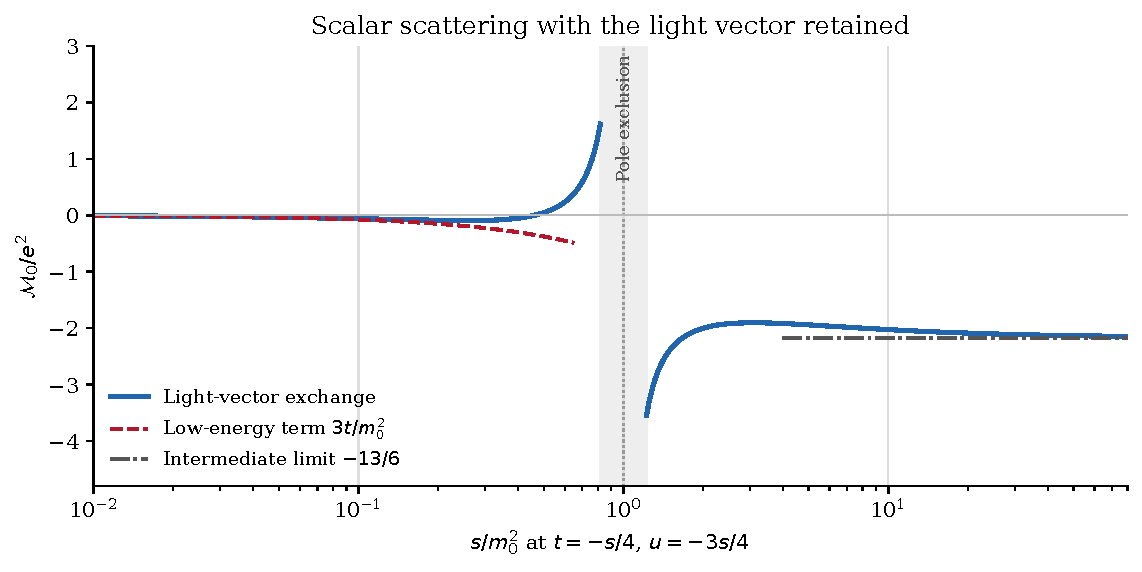
\includegraphics[width=.94\textwidth]{figures/output/threshold_amplitude.pdf}
\caption{The explicit amplitude \eqref{eq:modelamplitude} at fixed angle,
with $b/a=0.1$, $\theta_H=0.8$ and $\delta=0.1$. The shaded interval
is excluded by the light-pole separation. The low-energy curvature term
and the intermediate limit describe different parts of the allowed
window. These are analytic finite-model curves; the actual amplitude
is compared with them by Theorem~\ref{thm:amplitude}, whose error
constant is not numerically evaluated.}\label{fig:threshold}
\end{figure}

\subsection{Uniform curvature of the selected plane}
There is also a geometric consequence of the same vertices. In real
unitary $L^2$ normalization the quotient curvature is
\begin{equation}\label{eq:spectralcurvature}
 K_{\mathbb R}=\sum_{n>0}\frac1{\mu_n}
 \left[3j_n^2+\sum_{\alpha=1}^3
 \left\{b_{n\alpha}(\mathsf u,\mathsf u)b_{n\alpha}(\mathsf v,\mathsf v)
              -b_{n\alpha}(\mathsf u,\mathsf v)^2\right\}\right].
\end{equation}
Indeed twice differentiating the moment equations gives second
fundamental form component $-b_{n\alpha}(w,z)/\sqrt{\mu_n}$ in
the normal direction $n_{n\alpha}$. The Gauss equation gives the
terms involving $b$. Differentiating the mechanical gauge connection
gives O'Neill's contribution $3\sum_n j_n^2/\mu_n$
\cite{oneill,bielawski,bielawski_erratum}.

This calculation applies at each fixed $b>0$ in a Sobolev slice of
the stable determinant-fixed $E$ block. Remove its ineffective
constant center. The gauge and moment-normal operators then have
bounded elliptic inverses at that point, defining the projections,
second fundamental form and $L^2$ Levi-Civita connection. Neutrality
removes the central cokernel; all other orthogonal-adjoint blocks
have zero vertices on this plane. The complete sums converge by the
fixed complementary gap and \eqref{eq:parsevalvertices}. Thus the
formula does not require a lower bound uniform in $b/a$ on the size
of that local slice.

\begin{proposition}\label{prop:uniformcurvature}
The sectional curvature of the actual harmonic bundle-moduli metric on the transported plane
\eqref{eq:plane}, with positive sign on a sphere, satisfies
\begin{equation}\label{eq:uniformcurvature}
 K_{\mathbb R}=\frac3{4b^2}[1+O(r^2)],\qquad
 K_{\gKS}=\frac3{2b^2}[1+O(r^2)],
\end{equation}
uniformly on \eqref{eq:hierarchycone}.
\end{proposition}
\begin{proof}
The light vector term in \eqref{eq:spectralcurvature} is
$3/(4b^2)[1+O(r^2)]$. The light normal terms are $O(r^4/b^2)$,
the other low terms are $O(r^4/a^2)$, and the complementary sum is
$O(1)$. Relative to $1/b^2$, each error is $O(r^2)$ or smaller.
The real unitary metric is twice the Dolbeault metric, so
$K_{\gKS}=2K_{\mathbb R}$.
\end{proof}

This result concerns the specified plane. It asserts neither bounded
derivatives of the full quotient metric nor uniform curvature control
on every plane. Appendix~\ref{sec:derivatives} gives a complementary
regular-patch derivative argument and an explicit singular horizontal
projector.

\section{A leading neutral-scalar interaction}\label{sec:scalar}

\subsection{Partial reduction on a regular patch}
Fix a relatively compact generic patch with $a,b>0$, and allow
the spectator bundle and K3 geometry to vary in small patches.
Write $z=(z_E,z_B)$ for bundle coordinates, $y$ for geometric
hypermultiplet coordinates, and $\chi^I$ for locally unwrapped
periodic two-form coordinates. The tensor multiplet and gravity
remain explicit. At energies below the smallest Higgs mass we
eliminate the three massive vector multiplets as well as the
gapped KK modes. We retain all unbroken gauge and charged matter
fields. The reduced scalar kinetic metric is a smooth gauged
target near this vacuum; it is not the possibly singular vacuum
quotient by the unbroken group.

The nondegeneracy needed for this partial reduction can be checked
in the local model. Let $D:\mathfrak{su}(2)\to T_xV$ be the
broken orbit map. At moment level zero its quaternionic images
obey
\begin{equation}\label{eq:normals}
 \langle I_\alpha D\xi,I_\beta D\zeta\rangle
                 =\delta_{\alpha\beta}Q_x(\xi,\zeta).
\end{equation}
The symplectic pairings of orbit vectors vanish by moment-map
equivariance. Since $D$ is injective, the three moment equations
have an invertible derivative on these nine real normal directions.
Their norm-square potential has positive Hessian there. The three
orbit directions are Goldstone directions; a local gauge slice
removes them. This accounts for the twelve real scalar directions
in the three massive vector multiplets.

At the actual ASD background the same construction has an elliptic
description. If $H$ is its full residual compact gauge group and
$\mathfrak h$ its parallel algebra, the hyperk\"ahler Weitzenb\"ock
formula identifies the ASD cokernel with
$\mathfrak h\otimes\RR^3$. On an $H$-invariant Coulomb slice the
complement of this cokernel has a bounded elliptic right inverse;
its finite kernel is the full retained ASD deformation space.
For an off-shell effective action solve the heavy
Euler--Lagrange equations on this complement. Their leading
linearization is the positive ASD Hessian. The implicit-function
construction gives a smooth $H$-equivariant solution in all retained
variables, with the unbroken moment maps left as a potential.
It agrees with the projected ASD construction on neutral ASD vacua;
these equations need not agree away from that locus. The metric,
two-form and fermionic complementary operators are those specified
in section~\ref{sec:vectors}. All inverse bounds here belong to
the fixed regular patch, and can deteriorate when its Higgs gap
vanishes.

The perturbative expansion below means the finite jet of this
tree action, order by order in $\eta$ and external derivatives.
The coefficient functions and the parameter derivatives actually
used are smooth on the fixed patch. The notation $\Oformal(\eta^j)$
specifies the absence of lower coefficients; it does not bound an
unconstructed infinite remainder at finite $\eta$.

\subsection{Mixed constraints and the vertical kinetic coefficient}
For a pure bundle velocity at fixed leading geometry, use a
parameter gauge connection $\Lambda_i$ and set
\begin{equation}\label{eq:horizontal-ASD}
 a_i=\partial_i\mathcal A-d_{\mathcal A}\Lambda_i,\qquad
 d_{\mathcal A}^*a_i=0,\qquad d_{\mathcal A}^+a_i=0.
\end{equation}
The external-index gauge equation is precisely the first condition;
$\mathcal A_\mu=\Lambda_i\partial_\mu z^i$ gives
$F_{\mu m}=a_{i,m}\partial_\mu z^i$. For stable determinant-fixed
$E,B$, the adjoint Laplacian is invertible off its retained central
kernel. Smooth slice dependence and elliptic differentiation control
$\Lambda_i$ and any fixed finite number of derivatives on the
patch. K3 geometric variations lift to nearby ASD connections:
the trace-free stable ASD cokernel is zero, since its harmonic
self-dual adjoint forms have parallel coefficients. The neutral
central equations are compatible with the fixed trivial determinants.

Put $f_i=\partial_i f$ and
$(j_i)_m=\BF(F_{mn},a_i{}^n)$. For the convention
$G_{\mu m}=\eta v_{i,m}\partial_\mu z^i$ the mixed Einstein
equation to the required order is
\begin{equation}\label{eq:Einsteinconstraint}
 \Delta_1v_i=df_i+j_i,\qquad d^*v_i=0.
\end{equation}
Its coefficients follow directly from
\eqref{eq:heterotic-action}: the conformal internal metric contributes
$-3\eta\,df_i/2$, the dilaton contributes $+\eta\,df_i$,
the mixed metric contributes $\eta d^*dv_i/2$, and the gauge
stress contributes $-\eta j_i/2$. The $H$ stress starts at
$\eta^2$; the mixed $R^2$ source for a pure bundle velocity does
also, because the leading tangent connection is independent of $z$.

The longitudinal equation is essential. Differentiating
\eqref{eq:Poisson}, using the Yang--Mills equation and trace invariance,
gives
\begin{equation}\label{eq:longitudinal}
 \Delta_0f_i=\tfrac12\BF(F_{mn},(d_{\mathcal A}a_i)^{mn})
 =\BF(F_{mn},D^ma_i{}^n)=-d^*j_i.
\end{equation}
Thus $df_i+j_i$ is co-closed. Since $H^1(S,\RR)=0$,
\eqref{eq:Einsteinconstraint} has the controlled solution
$v_i=\Delta_1^{-1}(df_i+j_i)$.

For the two-form constraint, write $H_S=\eta h_1$ and
$H_{\mu mn}=\eta(\mathcal H_i)_{mn}\partial_\mu z^i$.
The mixed Bianchi identity and the external-index two-form equation
give
\begin{equation}\label{eq:Bconstraint}
 d\mathcal H_i=\partial_i h_1+\BF(a_i\wedge F)=:S_i,
 \qquad d^*\mathcal H_i=0.
\end{equation}
The source is closed: the derivative of the internal Bianchi
identity is $d\partial_i h_1=-\BF(d_{\mathcal A}a_i\wedge F)$,
and the second term cancels it using $d_{\mathcal A}F=0$.
Since $H^3(S,\RR)=0$, with $G_3$ the ordinary Green operator,
\begin{equation}\label{eq:Bsolution}
 \mathcal H_i=d^*G_3S_i+h_i,
\end{equation}
where $h_i$ is harmonic. These harmonic components describe the
retained periodic two-form coordinates and their local connection;
they are not inverted. Their parameter-space curvature is the
harmonic projection of the universal Chern--Weil form, including
the parameter legs of the universal gauge connection. The universal
Bianchi identity makes it closed. On a contractible patch a smooth
connection potential is obtained by the Poincar\'e homotopy operator.
This accounts for parameter integrability; setting every $h_i$ to
zero independently would not do so. All computed coefficients
and their finite parameter derivatives are bounded on the patch.

The action now determines the leading bundle tensor, not merely its
expected scale. The mixed Yang--Mills term is order $\eta$ and gives
the $L^2$ metric of \eqref{eq:horizontal-ASD}. The leading metric and
dilaton are independent of $z$; their bundle dependence and metric
compensator start at order $\eta$, so their pure-bundle kinetic
contribution starts at $\eta^2$. The two-form constraint has the
same order, with its periodic-coordinate connection of order one.
The leading tangent connection is independent of $z$; its
variation through the corrected metric and torsion starts at
$\eta$. The curvature-squared and Lorentz Chern--Simons terms
therefore do not add an order-$\eta$ pure-bundle tensor. They are
not omitted from base and higher-order coefficients.

If $a_i=\beta_i-\beta_i^*$ with $\beta_i$ its $(0,1)$ part,
the real one-form norm is twice the Dolbeault norm. Restoring the
normalization \eqref{eq:YMaction} gives
\begin{equation}\label{eq:physicalmetric}
 S_{\rm scalar}=-\frac12\int C_B\gKS_{ij}
               \partial_\mu z_E^i\partial^\mu z_E^j+\cdots,
 \qquad C_B=\frac{2L^2}{g_{10}^2}.
\end{equation}
This is a block of the full kinetic tensor, not yet its intrinsic
or ambient curvature.

\subsection{The other neutral fields and ambient curvature}
After a common six-dimensional normalization, the neutral metric
has the following finite-order structure:
\begin{align}\label{eq:blockmetric}
 G_\eta={}&g_{AB}(y)dy^A dy^B
 +\eta h_{ij}(y,z)(dz^i+C_A^i dy^A)(dz^j+C_B^jdy^B)\nonumber\\
 &+\eta^2 k_{IJ}(y)(d\chi^I+V^I)(d\chi^J+V^J)+E_\eta,
 \\
 h(y,z)={}&V_0^{-1}\bigl(g^{\rm KS}_{E,y}(z_E)
                               \oplus g^{\rm KS}_{B,y}(z_B)\bigr).
 \label{eq:productbundle}
\end{align}
The leading blocks $g,h,k$ are positive and smooth. The connection
$V$ has both $dy$ and $dz$ components. Perturbative two-form shift
symmetry makes the coefficient functions independent of $\chi$.
With two parameter derivatives, the formal remainder orders are
\begin{equation}\label{eq:blockorders}
 \begin{gathered}
 E_{yy}=\Oformal(\eta),\quad
 E_{yz},E_{zz}=\Oformal(\eta^2),\\
 E_{y\chi},E_{z\chi},E_{\chi\chi}=\Oformal(\eta^3).
 \end{gathered}
\end{equation}
The leading $y,z$ cross term is included in $C$.
The leading two-form Hodge metric depends only on $y$; its
first correction is one order higher. These orders follow from
the constraints and action count above and agree with the
geometry--bundle--two-form hierarchy of \cite{alpv}. The Lorentz
Chern--Simons and curvature-squared contributions identified there
are included at their required orders.

We spell out the curvature consequence because the small axion
block cannot be treated as a bounded spectator. In the coframe
of \eqref{eq:blockmetric} the scales are $(1,\eta,\eta^2)$.
In coordinates the inverse orders are
\begin{gather*}
 G^{yy}=O(1),\quad G^{yz}=O(1),\quad
 G^{zz}=\eta^{-1}h^{-1}+O(1),\\
 G^{z\chi}=O(\eta^{-1}),\quad G^{y\chi}=O(1),\quad
 G^{\chi\chi}=O(\eta^{-2}).
\end{gather*}
For lower-index Christoffel symbols with two bundle arguments,
\[
 \Gamma_{z,zz}=\eta\Gamma(h)_{z,zz}+O(\eta^2),\quad
 \Gamma_{y,zz}=O(\eta),\quad \Gamma_{\chi,zz}=O(\eta^2).
\]
The last estimate uses shift independence. In the coordinate
curvature formula the second-derivative terms and the $zz$
Christoffel contraction give $\eta R(h)$; all other contractions
have order $\eta^2$ or higher, including the one with
$G^{\chi\chi}$. Consequently
\begin{equation}\label{eq:ambientleading}
 R(G_\eta)_{EEEE}=\frac\eta{V_0}R(g_E^{\rm KS})
                                  +\Oformal(\eta^2).
\end{equation}
The leading product in \eqref{eq:productbundle} is essential for
the pure-$E$ coefficient. The spectator-bundle moduli have not
been declared constant. A nonsingular tensor-field block can
also be retained; its four-$E$ contributions start one order
later by the same calculation. In product-frame units the leading
sectional curvature is therefore $C_B^{-1}K_{\gKS}$.

It remains to compare neutral curvature with the ambient scalar
target including charged fields. Every additional hypermultiplet
in table~\ref{tab:matter} is charged under the residual compact
group. The neutral fields are exactly the $E,B$ moduli and the
geometric/two-form fields. The equivariant partial reduction
constructed above gives a smooth metric on which the full residual
group acts by isometries. Its fixed component is totally geodesic:
a geodesic with fixed initial point and fixed tangent remains
fixed by uniqueness. Thus its four-neutral curvature is the
ambient scalar curvature. The residual global gauge action,
including shared centers, is retained; no further finite or
continuous quotient is taken. This argument does not say that
the $E$-only slice is totally geodesic among the neutral fields;
their effects have instead been included in
\eqref{eq:blockmetric}--\eqref{eq:ambientleading}.

\subsection{The interaction and its order of limits}
Combining \eqref{eq:physicalmetric}, \eqref{eq:ambientleading}
and Proposition~\ref{prop:curvature} proves
\eqref{eq:intro-curvature}. In physical scalar normal coordinates
with the convention assigning positive curvature to a sphere,
$G_{ij}=\delta_{ij}-\tfrac13R_{ikjl}\phi^k\phi^l+\cdots$.
The two-polarization part of the Lorentzian action
$-\tfrac12G_{ij}\partial\phi^i\partial\phi^j$ is
\begin{equation}\label{eq:interaction}
 \mathcal L_4=\frac{\mathcal K_{\rm phys}^{\rm lead}}6
 \left[(\phi^v)^2(\partial\phi^u)^2
       +(\phi^u)^2(\partial\phi^v)^2
       -2\phi^u\phi^v\partial\phi^u\cdot\partial\phi^v\right]
\end{equation}
at the calculated large-volume order. It is a nonzero
curvature-controlled scalar coefficient in the covariant tree
amplitude dictionary \cite{cheung}. Neutral exchange contributions
that appear in other coordinates assemble into this coefficient;
universal graviton-exchange poles are separate.

The statement first computes the leading tree large-volume
coefficient on a fixed regular patch, then takes
$a=\varepsilon$, $b=\kappa\varepsilon$ with fixed $\kappa>0$.
The geometric relative error is $O_\kappa(\varepsilon^2)$.
The derivative expansion requires
$E_{\rm probe}\ll\kappa\varepsilon/L$, with its next parameter
$E_{\rm probe}^2/m_{\min}^2$, and perturbative interactions in
canonical normalization. Taking the probe energy sufficiently
small and the ten-dimensional coupling weak leaves a nonempty
regime. Keeping a six-dimensional dilaton fixed as volume grows
need not keep that ten-dimensional coupling small, so these
limits are specified separately. We have not bounded higher
physical coefficients as $\varepsilon\to0$ or proved a uniform
simultaneous finite-$\eta$ curvature remainder.

\section{Partial results at the next heterotic tree order}\label{sec:nexttree}

The amplitude in Theorem~\ref{thm:amplitude} includes the complete
Yang--Mills tower. A further coefficient is required to include the
other heterotic interactions. We identify its perturbative order, bound
the quadratic potential mixing with K3 shape deformations, and calculate
the universal massless spin-two contribution. The remaining
coefficient is not evaluated here.

\subsection{Order counting and the required terms}
Remove the common gravitational prefactor and write the action in
reference internal units as
\begin{equation}\label{eq:treeorders}
 S[Y,\mathcal A]=S_0[Y]+\eta S_1[Y,\mathcal A]
             +\eta^2 S_2[Y,\mathcal A]+\Oformal(\eta^3),
\end{equation}
where $Y$ denotes the metric, dilaton and two-form. The term $S_1$
contains both Yang--Mills and tangent curvature squared. In the field
scheme of \eqref{eq:heterotic-action}, $S_2$ includes the terms generated
by the recursive Chern--Simons definition of $H$ and the composite
Hull connection. The absence of a new independent bosonic invariant
at this order does not set $S_2$ to zero
\cite[section~3.1]{aqs}\cite[section~2.1]{mcorist_yin,mcorist_picard}.

Each canonical gauge or connection-scalar external leg removes a factor
$\eta^{1/2}$ in these units. A bare term $\eta^nS_n$ with four such
legs has order $\eta^{n-2}$. The leading Yang--Mills amplitude has
order $\eta^{-1}$; its first relative-$\eta$ correction requires the
complete bare action through $\eta^2$. The same count follows for
exchange diagrams after canonical normalization of internal fields.
Independent bare $\eta^3$ terms affect a later coefficient at fixed
deformation and momentum. This order count gives no estimate uniform
in a vanishing Higgs mass or near a pole.

One can organize the calculation by the stationary action. Let $Y_0$
be the leading product background, $K$ the gauge-fixed Hessian of $S_0$,
and $J[\mathcal A]=\delta_Y S_1[Y_0,\mathcal A]$. With constraints,
zero modes and propagator boundary conditions specified, eliminating
the neutral fluctuations to this order would give
\begin{equation}\label{eq:stationarycorrection}
 W[\mathcal A]=S_2[Y_0,\mathcal A]
       -\tfrac12\langle J[\mathcal A],K_F^{-1}J[\mathcal A]\rangle.
\end{equation}
This follows by inserting the stationary displacement
$-\eta K_F^{-1}J$ into the quadratic leading action and its source.
The massless poles in $K_F^{-1}$ are retained; the expression is not
a local elimination of massless fields. At zero external momentum,
the compatible complementary inverse is used, with background zero
modes fixed by the stated normalization.

Formula~\eqref{eq:stationarycorrection} is an organization of the
missing calculation, not a computed amplitude. If $J_d$ is the
degree-$d$ fluctuation part, its quartic term involves
$J_0K_F^{-1}J_4$, $J_1K_F^{-1}J_3$ and
$\tfrac12J_2K_F^{-1}J_2$. The first two include the corrected background
and linear mixing. One must also insert the cubic part of $W$ into
Yang--Mills exchange diagrams, insert its quadratic part into internal
propagators, and correct the external modes and residues. Adding only
neutral exchange between two scalar-pair sources omits these terms.
The scalar constraints in section~\ref{sec:scalar} and the vector pencil
in section~\ref{sec:coupled} supply parts of this reduction, but neither
determines the complete cubic and quartic vertices.

\subsection{Quadratic mixing with K3 metric deformations}
One part of the coupled reduction admits a relative estimate from the
same harmonic energy bound. Consider a volume-preserving infinitesimal
hyperk\"ahler metric deformation in harmonic gauge, modulo
diffeomorphisms and rotations of the parallel self-dual triple.
Its period variations are harmonic ASD two-forms
$\beta_\alpha=(\partial_\tau\omega_\alpha)^-$; this is the usual
$\mathbb R^3\otimes\mathcal H^-_2(S)$ description of the 57-dimensional
space of K3 shape tangents \cite{gik}. Normalize
$\sum_\alpha\|\beta_\alpha\|^2\le1$.

At fixed connection, put $f_\alpha=\partial_\tau\mu_\alpha$ and
$c_{n\alpha}=\langle p_n,f_\alpha\rangle$. Up to the fixed component
signs in \eqref{eq:infinitemoments}, the source is
$f_\alpha=*_0(F\wedge\beta_\alpha)$. The variation of the outer
Hodge star contributes zero because $F\wedge\omega_\alpha=0$ at the
ASD background, and the self-dual part of the period variation wedges
to zero with $F$. Since $\beta_\alpha$ is harmonic and ASD,
\begin{equation}\label{eq:shapesource}
 |c_{n\alpha}|
 =\left|\int_S\BF(p_n,F)\wedge\beta_\alpha\right|
 =\left|\langle\HH_2\BF(p_n,F),\beta_\alpha\rangle\right|.
\end{equation}

\begin{lemma}\label{lem:shapemixing}
For each low positive mode,
\begin{equation}\label{eq:shapemixing}
 \sum_\alpha|c_{n\alpha}|^2\le Cr^2\mu_n.
\end{equation}
The mixed Hessian of $\tfrac12\sum_\alpha\|\mu_\alpha\|^2$
between the unit scalar normal $n_{n\alpha}$ and this metric tangent
is $\sqrt{\mu_n}c_{n\alpha}$, hence is $O(r\mu_n)$.
The normal gauge-field adjustment to the linearized ASD equation is
\begin{equation}\label{eq:shapelift}
 \dot{\mathcal A}_\perp
 =-\sum_{n>0,\alpha}\frac{c_{n\alpha}}{\sqrt{\mu_n}}n_{n\alpha}.
\end{equation}
Its low component is $O(r)$ and its complementary component is $O(1)$
in every fixed spatial Sobolev norm, uniformly in $b/a$.
\end{lemma}
\begin{proof}
Equations~\eqref{eq:shapesource} and~\eqref{eq:relativeharmonic}
give \eqref{eq:shapemixing} by Cauchy--Schwarz. They also show that
the source has zero projection on every parallel zero-form.
At zero moment level the potential Hessian is the pairing of first
moment derivatives. Equation~\eqref{eq:quaternionicgram} gives the
displayed mixed entry and verifies that \eqref{eq:shapelift} solves
$D\mu_\alpha(\dot{\mathcal A}_\perp)+f_\alpha=0$.

For the full adjoint ASD complex the moment-map cokernel consists of
three copies of the parallel algebra; the preceding vanishing removes
each compatibility obstruction. The full lift includes the spectator
$B$ connection's curvature source and its gapped response. In a
trace-free determinant-fixed stable $E$ block the obstruction space
is zero; restricting the lift to that block means restricting the
source as well.

Orthonormality of the normals gives
\[
 \|\dot{\mathcal A}_{\perp,\mathrm{low}}\|^2
 =\sum_{n\,\mathrm{low},\alpha}\frac{|c_{n\alpha}|^2}{\mu_n}
 \le Cr^2.
\]
Each unit low normal solves the uniformly elliptic ASD one-form
square with bounded eigenvalue. Its coefficients are uniformly
smooth in the fixed unitary presentation, so elliptic regularity
bounds the normal in every fixed $H^s$ norm. The finite low sum
therefore has the same $O(r)$ bound in $H^s$; dividing a spatial
estimate for $Dp_n$ by a small $\sqrt{\mu_n}$ is unnecessary.
For the complementary part, Parseval and the fixed positive gap
give a uniform $L^2$ bound. The curvature and normalized harmonic
$\beta_\alpha$ have uniformly bounded spatial derivatives, so the
source does also. The complementary ASD equation and elliptic
regularity then give its fixed-$H^s$ bounds.
\end{proof}

In the common normalization of \eqref{eq:treeorders}, a canonical
gauge normal carries $\eta^{-1/2}$ and a geometry mode has leading
order-one normalization. Thus this potential block has a low mixed
entry $O(\sqrt\eta\,r\mu_n)$ and a static canonical normal
admixture $O(\sqrt\eta\,r)$. This controls one quadratic contribution.
It does not bound parameter derivatives of \eqref{eq:shapelift},
the full corrected kinetic form, or a two-external-scalar neutral
source at nonzero momentum. Those are still needed for the complete
four-point coefficient.

\subsection{The massless graviton and the angular domain}
Use the six-dimensional Einstein frame normalized to agree with the
product-frame external metric at the fixed leading vacuum. Define
\begin{equation}\label{eq:Einsteinnormalization}
 S_{\rm EH}=\frac1{2\kappa_6^2}\int\sqrt{-g}\,R,
 \qquad g_{\mu\nu}=\eta_{\mu\nu}+2\kappa_6h_{\mu\nu}.
\end{equation}
The curvature convention in this Lorentzian action gives the usual
healthy graviton propagator. For canonical orthogonal massless scalars,
the minimally coupled graviton vertex is diagonal in species. Hence
$\phi\chi\to\phi\chi$ has only $t$-channel graviton exchange at
this order. It is
\begin{equation}\label{eq:gravitonamplitude}
 \mathcal M_{\rm grav}=\kappa_6^2\frac{su}{t}.
\end{equation}
For completeness, the conserved scalar stress at a vertex is
$T_{\mu\nu}(p,p')=p_\mu p'_\nu+p_\nu p'_\mu-\eta_{\mu\nu}p\cdot p'$.
The conserved-source propagator numerator in $D$ dimensions is
\[
 P_{\mu\nu,\rho\sigma}
 =\tfrac12(\eta_{\mu\rho}\eta_{\nu\sigma}
           +\eta_{\mu\sigma}\eta_{\nu\rho})
       -\frac{\eta_{\mu\nu}\eta_{\rho\sigma}}{D-2}.
\]
On-shell contractions give
$T_1PT_2=(s^2+u^2-t^2)/2=-su$. In mostly-plus signature the exchanged
momentum has $q^2=-t$, and the two vertices and propagator give
$\mathcal M=\kappa_6^2T_1PT_2/q^2=-\kappa_6^2T_1PT_2/t$, proving
\eqref{eq:gravitonamplitude} also in $D=6$. Conservation removes
longitudinal gauge terms.

Restoring the common normalization of \eqref{eq:heterotic-action},
the gauge term is
\[
 -\frac{\alpha'e^{-2\Phi_0}}{8\kappa_{10}^2}
                    \BF(F_{MN},F^{MN}).
\]
Comparison with \eqref{eq:YMaction} and integration over the leading
volume $V_0L^4$ give
\begin{equation}\label{eq:gravitycoupling}
 g_{10}^2=\frac{2\kappa_{10}^2e^{2\Phi_0}}{\alpha'},\qquad
 \kappa_6^2=\frac{\kappa_{10}^2e^{2\Phi_0}}{V_0L^4}
           =\frac34\alpha'e^2.
\end{equation}
These are the leading background normalizations needed for this
coefficient. If $|t|\ge\delta E^2$, then
\begin{equation}\label{eq:gravitybound}
 |\mathcal M_{\rm grav}|
 \le\frac{3}{4\delta}e^2\eta(EL)^2.
\end{equation}
At $E\asymp b/L$ this is $O(e^2\eta b^2)$, uniformly in $b/a$.
It is an absolute bound relative to the natural amplitude scale $e^2$,
not a relative bound against a Yang--Mills amplitude that may vanish.

The massless pole requires a change to the domain of any full-amplitude
comparison. For sufficiently small nonzero $s$, the domain
\eqref{eq:amplitudedomain} allows $t\to0$ with $u\to-s$.
The graviton term then has the nonzero residue $-\kappa_6^2s^2$.
Thus the pure-Yang--Mills comparison cannot be extended to the
unsubtracted full amplitude on precisely the same forward-allowed
domain by appending a bounded error. Angular separation from massless
poles, or a specified gauge-invariant pole subtraction, is necessary.
This restriction does not by itself control the other terms of
\eqref{eq:stationarycorrection}.

The unresolved part is the complete constrained neutral-field source,
its recursively induced contacts, the corrected scalar external states,
and their combined exchanges and residues. Uniform estimates would
also have to control small gauge inverses and mass insertions in this
sum. They do not follow from the fixed complementary gaps alone.
Even a complete calculation of this coefficient would remain distinct
from a bound on the full finite-$\alpha'$ remainder.

\section{Discussion}\label{sec:discussion}

The compactification constructed here has a local region in which
one can compare actual HE geometry with two physically identified
quantities. The leading vector hierarchy is controlled relatively
even when its smallest scale is arbitrarily weaker than the
others. The defined first-order tree pencil includes the leading
metric and two-form vector towers, and its ASD cancellation
preserves the full unbroken kernel. The scalar calculation uses
the same family, but requires derivative estimates and a compensated
reduction to identify a leading ambient interaction coefficient.
Its angular restriction is essential.

The two results have different uniformity. The spectral theorem
uses energy-relative reconstruction and survives changing orbit
scales without differentiating a horizontal projector. Curvature
uses smooth holomorphic regularity on a fixed angular patch.
The explicit projector derivatives and nonzero cone curvature
show why a uniform derivative assertion needs further information.
A quantitative lower bound on the admissible holomorphic chart
scale would be one route toward such a result.

The hyperk\"ahler quotient, qualitative Higgs mechanism,
heterotic bundle kinetic term, Hodge decomposition and
curvature--amplitude relation are established ingredients. The
substantial analytic premise is the local relative comparison
in \cite{wuebben15}; the present contribution is its normalized,
coupled use in an actual compactification with a worked interaction
and explicit error regimes. The local harmonic argument from
\cite{wuebben20} supplies the needed coordinates without a global
claim for the rank-six moduli space.

Several stronger questions remain. An exact finite-$\alpha'$
background with numerical remainder estimates would be needed
to turn the vector pencil bound into an exact corrected-pole
bound. A simultaneous interaction theorem would require control
of higher physical coefficients and their derivatives near
enhancement. Finite-coupling corrections require separate estimates.
Nonzero-FI wall crossing, bubbling and quantum amplitudes are
also outside the present result. At energies above the smallest
Higgs mass, the three massive multiplets must be restored rather
than extending the quotient sigma model beyond its window.

\appendix
\section{The vector correction on a regular ray}\label{app:coefficient}

The estimate of Proposition~\ref{prop:coupled} admits an explicit
leading coefficient when $a=\varepsilon$, $b=\kappa\varepsilon$
with fixed $0<\kappa<1$. Use the fixed Coulomb presentation of
\eqref{eq:fixedcoulomb} and write
\[
 \alpha_\varepsilon=\varepsilon u+O(\varepsilon^2),\qquad
 C=[u,\cdot],\quad
 G=(Q_0D_0^*D_0Q_0)^{-1},\quad
 \Lambda=\Pi_0C^*C\Pi_0.
\]
Here $u$ is the first real harmonic deformation; all remainders
hold in each fixed spatial regularity. The fixed inverse $G$
maps $Q_0L^2$ to $Q_0W^{2,2}$, with its higher elliptic versions.
No second derivative of the finite balancing correction is used.

The low spectral space is a graph over $K_0=\ker D_0$.
Let $X_\varepsilon:K_0\to Q_0L^2$ be its graph map and set
\begin{equation}\label{eq:graphcoefficient}
 R=-GQ_0C^*C\Pi_0,\qquad
 U_\varepsilon=(I+X_\varepsilon)
              (I+X_\varepsilon^*X_\varepsilon)^{-1/2}.
\end{equation}
Then
\begin{equation}\label{eq:graphexpansion}
 X_\varepsilon=\varepsilon^2R+O(\varepsilon^3),\qquad
 U_\varepsilon=I+\varepsilon^2R+O(\varepsilon^3).
\end{equation}
Indeed \eqref{eq:lowcomplement} gives $X_\varepsilon=O(\varepsilon^2)$.
Writing the blocks of $D_\varepsilon^*D_\varepsilon$ as
$A_{00},B,L_Q$, Coulomb orthogonality gives
$B=\varepsilon^2Q_0C^*C\Pi_0+O(\varepsilon^3)$ and
$A_{00}=\varepsilon^2\Lambda+O(\varepsilon^3)$.
The graph equation
$L_QX+B=X(A_{00}+B^*X)$, with
$L_Q=L_{Q,0}+O(\varepsilon)$ between fixed elliptic spaces,
proves \eqref{eq:graphexpansion}. Elliptic regularity upgrades
the finite-dimensional graph estimate to every required spatial norm.
The isometric normalization changes the parallel component only
at order $\varepsilon^4$.

Let $f_0$ be the zero-mean solution of \eqref{eq:Poisson} at
the enhancement point, and let $h=\Delta_0^{-1}f_0$ have zero
mean, with $\Delta_0=-\nabla^2$. Define
\begin{align}
 Hk&=\HH_2\bigl(\BF(Rk,F_0)+\BF(k,u\wedge u)\bigr),
 \label{eq:Hcoefficient}\\
 \langle k,Wl\rangle
   &=\int_S h\,\BF([u,k],[u,l])\,dV_0 .
 \label{eq:Wcoefficient}
\end{align}
Internal one-form indices in the second equation are contracted
with $g_0$. The harmonic transgression \eqref{eq:transgression}
and \eqref{eq:graphexpansion} give
\begin{equation}\label{eq:masscoefficient}
 U_\varepsilon^*M_\varepsilon U_\varepsilon
      =\varepsilon^4H^*H+O(\varepsilon^5).
\end{equation}
The terms linear in a second connection coefficient are exact
under harmonic projection, which is why no such coefficient
appears in \eqref{eq:Hcoefficient}.

For the kinetic term, $\Pi_0f_\varepsilon\Pi_0=0$ exactly.
Since $f_\varepsilon=f_0+O(\varepsilon)$,
\[
 U_\varepsilon^*f_\varepsilon U_\varepsilon
 =\varepsilon^2(\Pi_0f_0R+R^*f_0\Pi_0)+O(\varepsilon^3)
 =-2\varepsilon^2W+O(\varepsilon^3).
\]
For the last equality use $G(f_0k)=hk$ for parallel $k$:
$D_0^*D_0(hk)=(\Delta_0h)k=f_0k$. Self-adjointness of $G$
then gives
$\langle k,f_0Rl\rangle=-\int h\,\BF([u,k],[u,l])$.

There is a further cancellation in the energy-dependent term.
Parallelness implies $[F_0,k]=0$, so trace invariance gives
$I_0^*[u,k]=0$ pointwise. Thus
\[
 J_\varepsilon U_\varepsilon
 =I_\varepsilon^*D_\varepsilon U_\varepsilon
 =O(\varepsilon^2).
\]
The resolvent term in $Z_\varepsilon$ is consequently
$O(\varepsilon^4)$ on the fixed interval. Combining these
identities yields
\begin{equation}\label{eq:coefficientlimit}
 \varepsilon^{-4}U_\varepsilon^*
 E_\varepsilon(\varepsilon^2z)U_\varepsilon
 \longrightarrow H^*H+2zW
\end{equation}
uniformly for $z$ in compact sets. This is an operator statement
and remains valid at a repeated leading eigenvalue.

For the three simple positive branches let $k_j$ be the unit
$\Lambda$ eigenvectors with
$\ell_j=8(\kappa^2,1,1+\kappa^2)_j/(3V_0)$, and define
\begin{equation}\label{eq:sigmacoefficient}
 \sigma_j=\|Hk_j\|^2+
       2\ell_j\int_S h\,|[u,k_j]|^2\,dV_0.
\end{equation}
If $\mu_{\varepsilon,j}$ denotes the corresponding actual
leading gauge eigenvalue, the roots of \eqref{eq:pencil} obey
\begin{equation}\label{eq:raycorrection}
 \lambda_{\varepsilon,j}^{[1]}(\eta)-\mu_{\varepsilon,j}
 =\eta\varepsilon^4\sigma_j
 +O_\kappa(\eta\varepsilon^5+\eta^2\varepsilon^6).
\end{equation}
To justify the remainder, pull the normalized leading eigenvector
back by $U_\varepsilon$. Its distance from $k_j$ is
$O_\kappa(\varepsilon)$ and its spectral separation is at least
$c_\kappa\varepsilon^2$. Differentiating the simple pencil root
at $\eta=0$ gives
$\lambda'_j(0)=\langle p_j,E_\varepsilon(\mu_j)p_j\rangle$.
Equation~\eqref{eq:coefficientlimit} gives
$\lambda'_j(0)=\varepsilon^4\sigma_j+O_\kappa(\varepsilon^5)$.
On the low-root interval,
$E=O(\varepsilon^4)$, $E_\lambda=O(\varepsilon^2)$ and
$E_{\lambda\lambda}=O(\varepsilon^4)$. The separated eigenvector
equation therefore gives $\partial_\eta p_j=O_\kappa(\varepsilon^2)$
and $\partial_\eta^2\lambda_j=O_\kappa(\varepsilon^6)$.
Taylor's theorem in $\eta$ proves \eqref{eq:raycorrection}.

The Pauli family has an additional selection rule. Write
$u=U\otimes\sigma_3+\kappa V\otimes\sigma_1$, with $U,V$
fixed unitary adjoint-valued one-forms on $A$. For the generators
$\widetilde k_i=I_A\otimes i\sigma_i/\sqrt{6V_0}$,
\begin{equation}\label{eq:selectionrule}
 H\widetilde k_1=H\widetilde k_3=0.
\end{equation}
Products in $u\wedge u$ have multiplicity factors in
$\operatorname{span}\{I,\sigma_2\}$, so their pairings with
$\widetilde k_1,\widetilde k_3$ vanish. For these two inputs,
the double commutator $C^*C\widetilde k_i$ has multiplicity
factors only in $\operatorname{span}\{\sigma_1,\sigma_3\}$.
The fixed complementary projection and Green operator preserve
that subspace; pairing with $F_A\otimes I$ is again zero.
This proves both terms of \eqref{eq:Hcoefficient} vanish.
The smallest and middle branches thus have only the warping
integral in \eqref{eq:sigmacoefficient}.

The formula determines a background-dependent coefficient, not
a universal nonzero number. Its value requires the reference ASD
fields and normalized harmonic representatives. Zero mean does
not give the warping integral a sign. At $\kappa=1$, individual
branch coefficients require the geometric splitting on the
repeated leading eigenspace as well as \eqref{eq:coefficientlimit}.
Finally \eqref{eq:raycorrection} concerns the defined pencil:
its powers of $\eta$ do not bound uncomputed string corrections.

\section{Regular-patch derivatives and the quotient model}\label{sec:derivatives}

\subsection{Preserving the quadratic rate in holomorphic coordinates}
The direct spectral proof in section~\ref{sec:scattering} controls the
selected curvature uniformly in $b/a$. A complementary approach on
regular angular patches upgrades \eqref{eq:metriccomparison} to metric
derivative estimates. Its quadratic rate cannot simply be differentiated;
the additional input is that both metrics are Ricci-flat K\"ahler in
the same complex structure.

\begin{lemma}\label{lem:interior}
Let $g_*$ be a smooth Ricci-flat K\"ahler metric on a complex manifold
$U$, and let $K\Subset U_1\Subset U$. Suppose $g_t$ are Ricci-flat
K\"ahler for the same complex structure and
$\sup_{U_1}|g_t-g_*|_{g_*}\le e_t\to0$. Then for every fixed
integer $k\ge0$ and $0<\alpha<1$,
\begin{equation}\label{eq:interior}
 \|g_t-g_*\|_{C^{k,\alpha}(K,g_*)}\le C_{K,U_1,g_*,k,\alpha}e_t
\end{equation}
for all sufficiently small $t$. The comparison uses the original
complex coordinates, without a parameter-dependent coordinate change.
\end{lemma}
\begin{proof}
Cover $K$ by finitely many fixed holomorphic coordinate balls compactly
contained in larger balls in $U_1$. Uniform metric equivalence and
\cite[Proposition~2.1]{hein_tosatti} give uniform bounds for every
fixed coordinate derivative on intermediate balls. These estimates
alone do not preserve the rate $e_t$.

For a Ricci-flat K\"ahler metric, differentiation of $\log\det g$
and the K\"ahler interchange of derivatives give
\begin{equation}\label{eq:RFsystem}
 g^{p\bar q}\partial_p\partial_{\bar q}g_{i\bar j}
 =g^{p\bar q}g^{r\bar s}
  (\partial_i g_{p\bar s})(\partial_{\bar j}g_{r\bar q}).
\end{equation}
Subtract the equations for $g_t$ and $g_*$, and write $h=g_t-g_*$.
The inverse difference is $g_*^{-1}-g_t^{-1}=g_t^{-1}hg_*^{-1}$.
Integrating the differential of the quadratic right side along
$g_*+sh$, $0\le s\le1$, gives a homogeneous linear system
\begin{equation}\label{eq:homogeneous}
 g_t^{p\bar q}\partial_p\partial_{\bar q}h
                      =A_t\cdot Dh+B_t h.
\end{equation}
$D$ here includes all real first derivatives. The principal symbol
is scalar times the identity on Hermitian components. Its ellipticity
and all needed coefficient norms are uniform on intermediate balls
by the preceding regularity estimate.

For clarity, lower-order coupling does not require a maximum
principle for a system. Apply scalar interior Schauder estimates
componentwise in the usual boundary-distance-weighted H\"older norms
on an intermediate ball. They give
\[
 |h|^*_{2,\alpha}\le C\|h\|_0+
 C_1\bigl(|h|^*_{1,\alpha}+|h|^*_{0,\alpha}\bigr).
\]
Weighted interpolation bounds the parenthesis by
$\delta |h|^*_{2,\alpha}+C_\delta\|h\|_0$.
Choose $C_1\delta<1/2$ and absorb. The weights are bounded below
on a smaller ball, yielding the ordinary $C^{2,\alpha}$ bound
by $\|h\|_0\le e_t$. Differentiating \eqref{eq:homogeneous}
and using nested balls gives each higher order inductively, since
every differentiated forcing term has the already established rate.
The finite cover proves \eqref{eq:interior}.
\end{proof}

Let $\delta_\varepsilon$ be cone dilation and put
\begin{equation}\label{eq:rescaled}
 g_\varepsilon=\varepsilon^{-2}\delta_\varepsilon^*\Psi^*\gKS.
\end{equation}
On any compact subset $K$ of the smooth-simple annulus
$\Cone\cap\{1/4<r<4\}$, both $g_\varepsilon$ and $\gC$ are
Ricci-flat K\"ahler in the same holomorphic chart. Equation
\eqref{eq:metriccomparison}, on a slightly larger regular neighborhood,
and Lemma~\ref{lem:interior} give
\begin{equation}\label{eq:all-derivatives}
 \|g_\varepsilon-\gC\|_{C^{k,\alpha}(K,\gC)}
                         \le C_{K,k,\alpha}\varepsilon^2.
\end{equation}
This is a standard elliptic consequence of the imported quadratic
comparison, not a new general regularity theorem.

The dependence on the smooth chart can also be made explicit.
Call a holomorphic embedding
$\varphi:B_{\CC^n}(0,2)\to\Cone_{\rm simple}$ admissible at
scale $0<\rho\le1$ if its image lies in $1/4<r<4$ and
\begin{equation}\label{eq:chartscale}
 \Lambda^{-1}g_{\rm Eucl}\le\rho^{-2}\varphi^*\gC
                                     \le\Lambda g_{\rm Eucl}
\end{equation}
for a fixed $\Lambda$. Apply the same proof to the two pulled-back
metrics divided by $\rho^2$. The reference derivatives are uniformly
bounded by the same local Ricci-flat estimate, so at the chart center
\begin{align}\label{eq:weighted}
 |\nabla^k(g_\varepsilon-\gC)|_{\gC}
   &\le C_k\varepsilon^2\rho^{-k},\\
 |\Rm(g_\varepsilon)-\Rm(\gC)|_{\gC}
   &\le C\varepsilon^2\rho^{-2}.\nonumber
\end{align}
Use the same tensor type on both sides of the curvature difference.
No lower bound for this admissible $\rho$ in terms of $b/a$ is
asserted. Such a lower bound, not merely the existence of very small
charts, would be needed to turn \eqref{eq:weighted} into an explicit
estimate uniform toward the Pauli axis.

\subsection{What fails near a changing stabilizer}
There is a direct diagnostic within the balanced locus. Add
$X_3=c\sigma_2$ to \eqref{eq:pauli}, with $a,b,c$ real and
$Y=0$. On the real two-plane of components
$(X_2\sigma_2,X_3\sigma_1)$, the orthogonal projection onto the
orbit of $i\sigma_3$ is
\begin{equation}\label{eq:projector}
 P(b,c)=\frac1{b^2+c^2}
 \begin{pmatrix}b^2&-bc\\-bc&c^2\end{pmatrix}.
\end{equation}
The other orbit generators occupy mutually orthogonal component
planes. At $c=0$,
\begin{equation}\label{eq:projectorderivatives}
 \partial_cP=\begin{pmatrix}0&-b^{-1}\\-b^{-1}&0\end{pmatrix},
 \qquad
 \partial_c^2P=\begin{pmatrix}-2b^{-2}&0\\0&2b^{-2}\end{pmatrix}.
\end{equation}
Their operator norms are $b^{-1}$ and $2b^{-2}$. Thus the
horizontal projection in the original balanced coordinates is not
uniformly $C^2$ as $b\to0$. This does not invalidate the relative
$C^0$ tensor comparison, and alone it is not an intrinsic curvature
calculation. The following calculation supplies the latter.

\subsection{Curvature in additional harmonic deformation directions}
At a Pauli point with $a,b>0$, let $u,v$ be the two Dolbeault
vectors in \eqref{eq:plane}. They are orthonormal for
\eqref{eq:flatmetric}. Their support is orthogonal to the orbit
and its three quaternionic images, so they are horizontal tangent
vectors to the hyperk\"ahler quotient.

\begin{proposition}\label{prop:curvature}
With curvature sign positive on a round sphere,
\begin{equation}\label{eq:conecurvature}
 K_{\gC}(u,v)=\frac3{2b^2}.
\end{equation}
For $a=\varepsilon$, $b=\kappa\varepsilon$ at fixed
$0<\kappa\le1$, transport this plane by $\Psi$ and normalize
using the actual harmonic metric. Its sectional curvature satisfies
\begin{equation}\label{eq:actualcurvature}
 K_{\gKS}=\frac3{2\kappa^2\varepsilon^2}+O_\kappa(1).
\end{equation}
\end{proposition}
\begin{proof}
The effective $\PU(2)$ action is free at this point and the moment
map is a submersion. Its zero set $N$ is a smooth submanifold of
the flat representation. Every tuple of Hermitian $X_j$ with
$Y=0$ lies in $N$. The affine plane $x+su+tv$ therefore lies
in $N$, and its three relevant second fundamental form entries
vanish. The Gauss equation gives $K_N(u,v)=0$.

Let $D_x\xi=([\xi,X_j],[\xi,Y_j])$ and use the bilinear
orbit Gram form $Q_x(\xi,\zeta)=\langle D_x\xi,D_x\zeta\rangle$,
viewed as a map from the Lie algebra to its dual. For horizontal
$u,v$, set $\beta(\xi)=\langle\xi\cdot u,v\rangle$.
Differentiating the one-form $\langle D_x\xi,\cdot\rangle$
gives $2\beta(\xi)$. Thus the curvature of the mechanical
connection is $2Q_x^{-1}\beta$, up to an irrelevant sign, and
the squared norm of O'Neill's tensor is $\beta(Q_x^{-1}\beta)$.
In the unnormalized basis $(i\sigma_1,i\sigma_2,i\sigma_3)$,
\begin{equation}\label{eq:orbitgram}
 Q_x=\operatorname{diag}(8a^2,8(a^2+b^2),8b^2),\qquad
 \beta=(0,0,-2).
\end{equation}
$Q_x$ here is the bilinear Gram matrix, not the matrix of
$D_x^*D_x$ after a Hilbert--Schmidt identification of the Lie
algebra with its dual. The resulting norm is $1/(2b^2)$.
O'Neill's formula \cite{oneill,bielawski} gives
$K_{N/\PU(2)}=K_N+3\|\mathcal A_{uv}\|^2$, proving
\eqref{eq:conecurvature}.

The ray with fixed $\kappa$ lies in a fixed regular angular patch;
its cone radius is $\sqrt{2(1+\kappa^2)}\varepsilon$.
The $C^2$ estimate \eqref{eq:all-derivatives} changes sectional
curvature of the rescaled metric by $O_\kappa(\varepsilon^2)$.
Scaling back gives \eqref{eq:actualcurvature}. In particular its
relative error is $O_\kappa(\varepsilon^2)$.
\end{proof}

Equation~\eqref{eq:actualcurvature} supplies an independent regular-ray
check of Proposition~\ref{prop:uniformcurvature}. The latter's direct
vertex proof also allows $b/a\to0$; the local derivative argument
above does not provide that additional uniformity. Section~\ref{sec:scalar}
identifies the leading physical coefficient while retaining the other
neutral fields.

\begin{figure}[t]
\centering
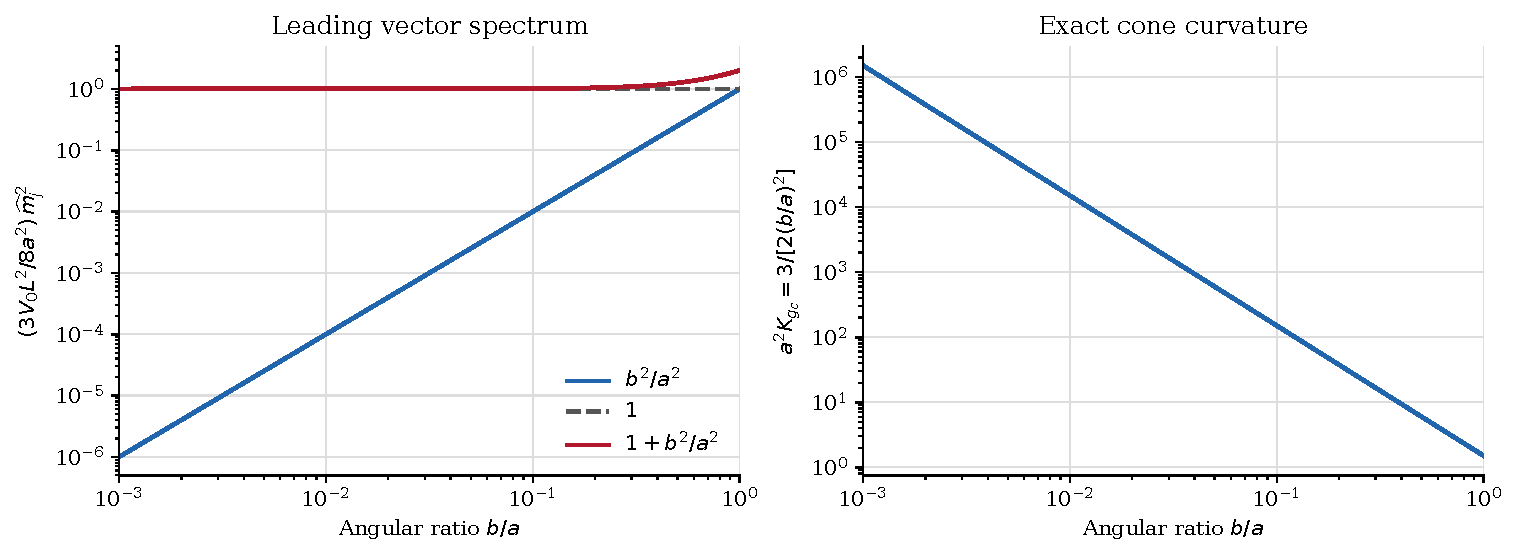
\includegraphics[width=\textwidth]{figures/output/finite_scales.pdf}
\caption{Exact finite-model formulas as the angular ratio decreases.
Left: the three normalized leading squared vector masses. The relative
geometric estimate remains uniform over the plotted ratios. Right:
the cone curvature of the horizontal two-plane \eqref{eq:plane}.
Proposition~\ref{prop:uniformcurvature} transfers this selected curvature
to the actual harmonic metric with uniform relative quadratic error for
$0<b\le\kappa_0a$, $\kappa_0<1$. Both panels
plot analytic formulas, not numerical HE solutions.}
\label{fig:scales}
\end{figure}

\bibliographystyle{JHEP-doi}
\bibliography{references}
\end{document}
